% !TEX root = ../main.tex

% 分析与讨论	
\begin{table}
	\renewcommand\arraystretch{1.7}
	\begin{tabularx}{\textwidth}{|X|X|X|X|}
		\hline
		Major：& Physics &Grade：& 2022\\
		\hline
		Name： & 杨舒云 & Student number：& 22344020 \\
		\hline
		Date：& 2024/10/25 & Score： &\\
		\hline
	\end{tabularx}
\end{table}
\section{APL1-1-A 电阻热噪声及玻尔兹曼常量测量 \\ Analysis \& Discussion}


%---------------------------------------------------------------------
% 数据处理
\subsection{Data Processing}

% 分析
\subsubsection{Analysis}
\begin{enumerate}
	\item 数据质量评定
	
	按照讲义要求，为了说明所采数据X或Y是随机噪声和X的采样是独立的，我们可以对采集到的数据进行如下分析：正则分布检、X-Y数据相关性和X或Y数据自相关性。我对现场测量和远程测量共18组数据都进了分析（相关代码见\textbf{附件}），\textbf{完整的绘图结果}见上传的数据文件，\textbf{部分结果}如下所示。
	
	\begin{enumerate}
		\item 对数据 \texttt{local\_Data1} 的 \(X\) 数据列进行正则分布检验，结果如下所示：
		
		\begin{itemize}
			\item \textbf{Shapiro-Wilk 检验}:
			\begin{itemize}
				\item 统计量: \(0.9997\), p 值: \(0.8419\)
				\item 结论: 数据符合正态分布假设 (p > 0.05)
			\end{itemize}
			
			\item \textbf{Kolmogorov-Smirnov 检验}:
			\begin{itemize}
				\item 统计量: \(0.0071\), p 值: \(0.9796\)
				\item 结论: 数据符合正态分布假设 (p > 0.05)
			\end{itemize}
			
			\item \textbf{简化卡方检验}:
			\begin{itemize}
				\item 简化卡方值: \(6.4167\)
				\item 结论: 数据符合正态分布假设 (卡方值 < 临界值)
			\end{itemize}
		\end{itemize}
		
		对数据 \texttt{local\_Data1} 的 \(Y\) 数据列进行正则分布检验，结果如下所示：
		
		\begin{itemize}
			\item \textbf{Shapiro-Wilk 检验}:
			\begin{itemize}
				\item 统计量: \(0.9995\), p 值: \(0.4022\)
				\item 结论: 数据符合正态分布假设 (p > 0.05)
			\end{itemize}
			
			\item \textbf{Kolmogorov-Smirnov 检验}:
			\begin{itemize}
				\item 统计量: \(0.0100\), p 值: \(0.7716\)
				\item 结论: 数据符合正态分布假设 (p > 0.05)
			\end{itemize}
			
			\item \textbf{简化卡方检验}:
			\begin{itemize}
				\item 简化卡方值: \(13.6612\)
				\item 结论: 数据符合正态分布假设 (卡方值 < 临界值)
			\end{itemize}
		\end{itemize}
		
		对数据 \texttt{local\_Data1} 进行相关性分析，结果如下所示：
		
		\begin{itemize}
			\item \textbf{Pearson 相关系数}:
			\begin{itemize}
				\item 系数: \(0.0117\), p 值: \(0.4393\)
				\item 结论: 在显著性水平 0.05 下，两列数据不存在显著的线性相关性 (p > 0.05)
			\end{itemize}
			
			\item \textbf{Spearman 相关系数}:
			\begin{itemize}
				\item 系数: \(0.0079\), p 值: \(0.5992\)
				\item 结论: 在显著性水平 0.05 下，两列数据不存在显著的非参数相关性 (p > 0.05)
			\end{itemize}
		\end{itemize}
		
		\begin{figure}[h!]
			\centering
			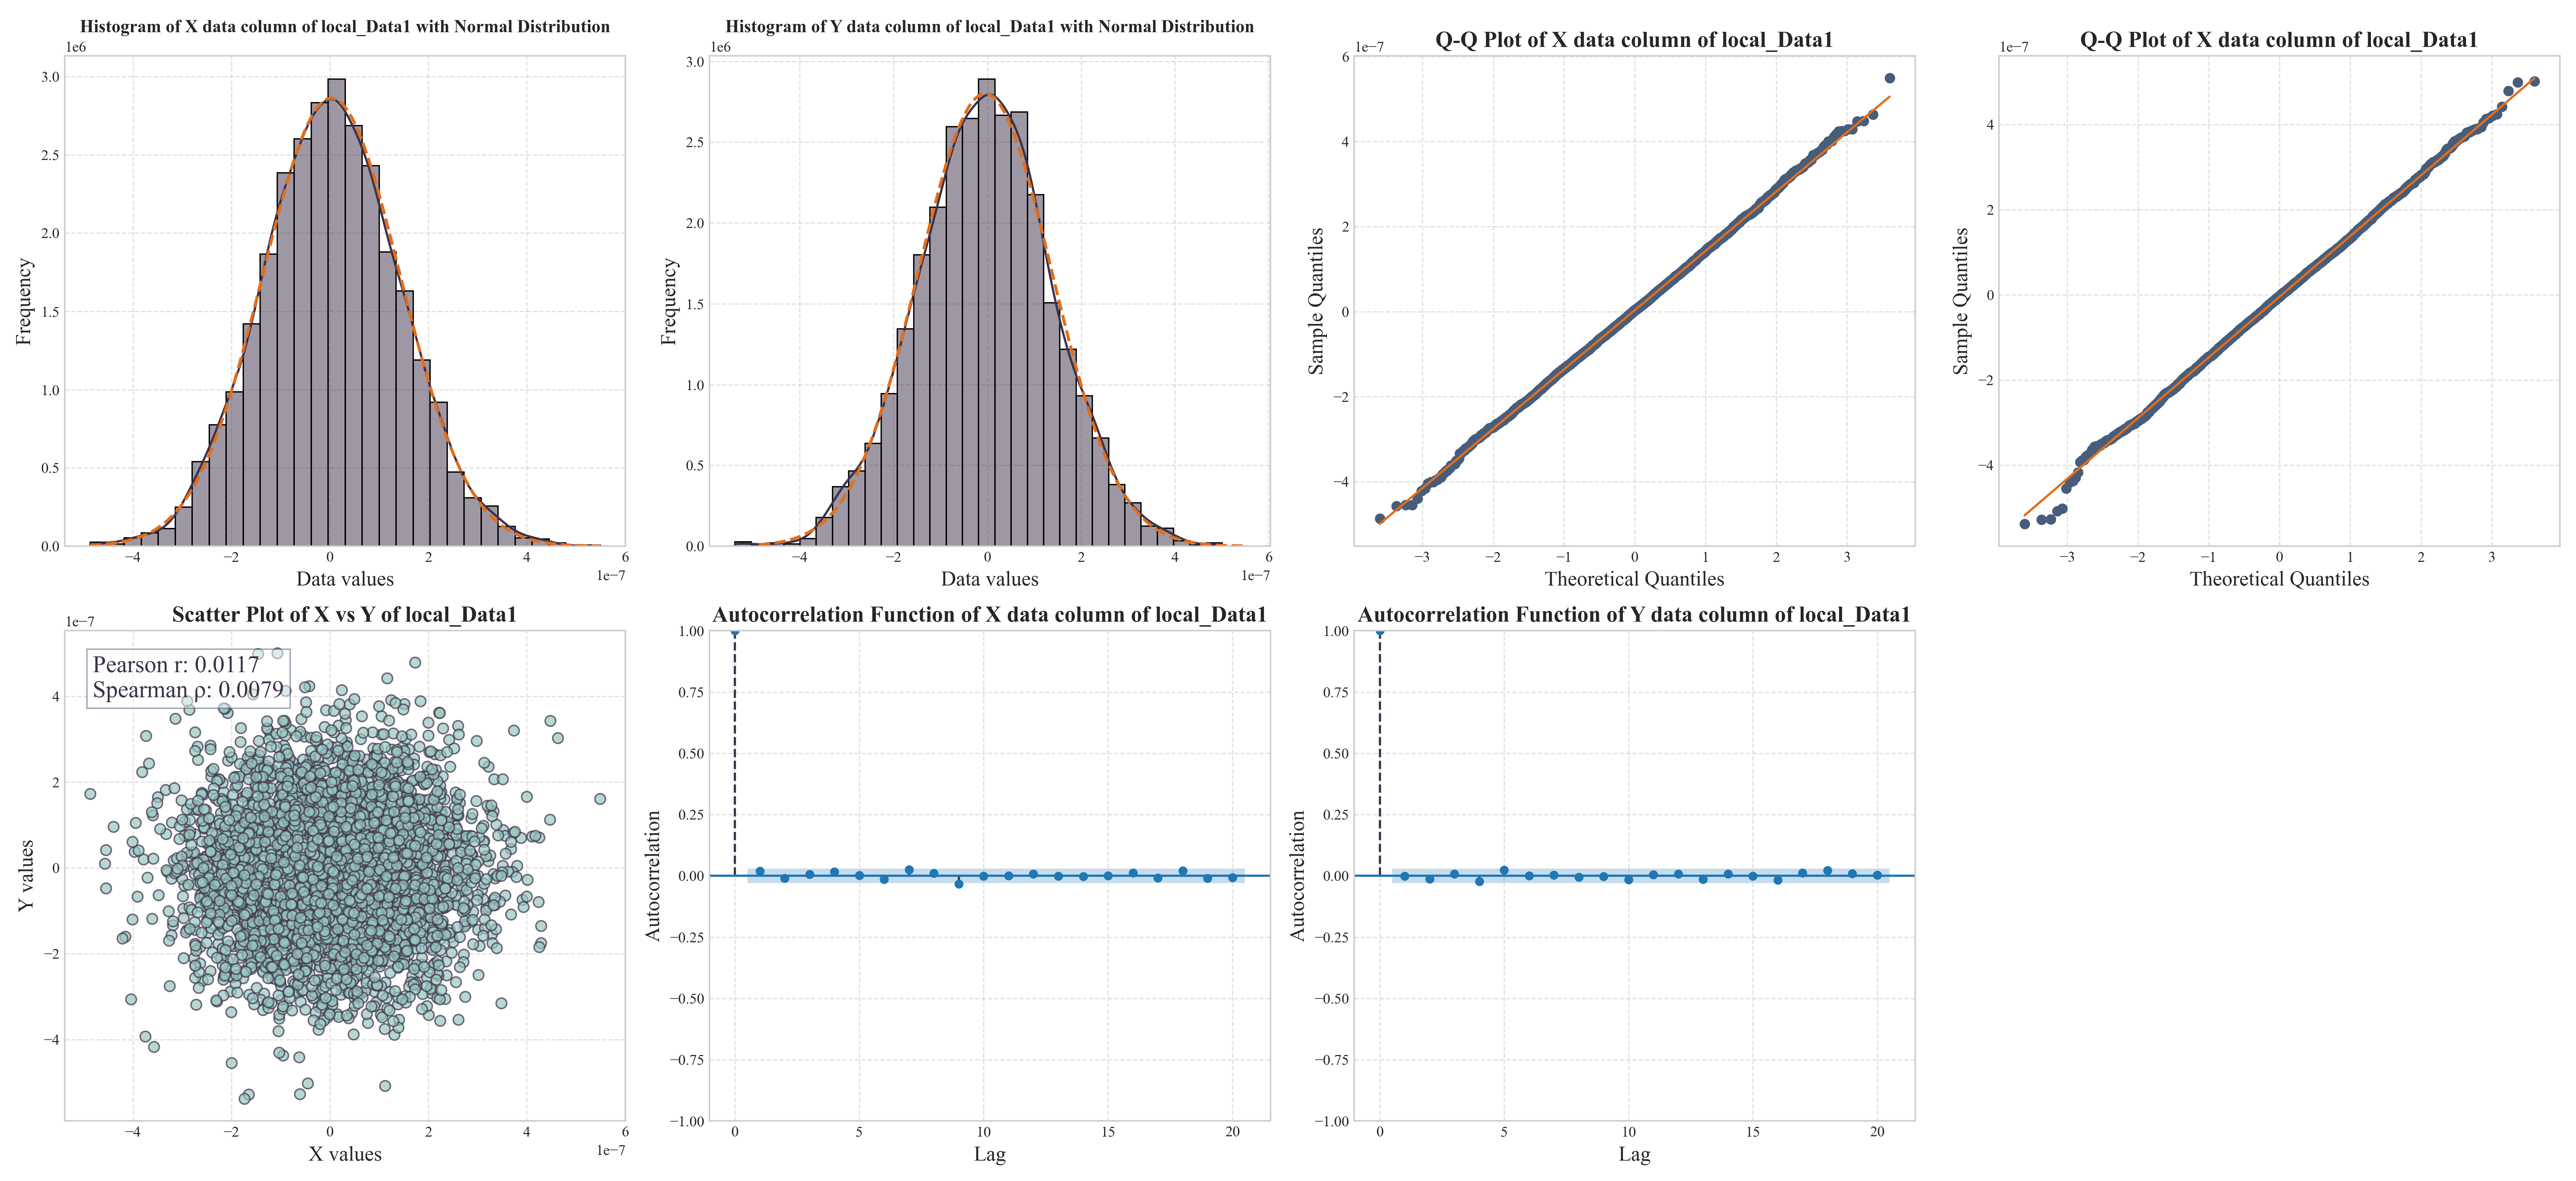
\includegraphics[width=\linewidth]{images/correlation-analysis-output/local_Data1}
			\caption{数据质量评定：现场测量Data1}
			\label{fig:localdata1}
		\end{figure}
		
		\item 对数据 \texttt{local\_Data2} 的 \(X\) 数据列进行正则分布检验，结果如下所示：
		
		\begin{itemize}
			\item \textbf{Shapiro-Wilk 检验}:
			\begin{itemize}
				\item 统计量: \(0.9997\), p 值: \(0.9246\)
				\item 结论: 数据符合正态分布假设 (p > 0.05)
			\end{itemize}
			
			\item \textbf{Kolmogorov-Smirnov 检验}:
			\begin{itemize}
				\item 统计量: \(0.0089\), p 值: \(0.9692\)
				\item 结论: 数据符合正态分布假设 (p > 0.05)
			\end{itemize}
			
			\item \textbf{简化卡方检验}:
			\begin{itemize}
				\item 简化卡方值: \(4.8212\)
				\item 结论: 数据符合正态分布假设 (卡方值 < 临界值)
			\end{itemize}
		\end{itemize}
		
		对数据 \texttt{local\_Data2} 的 \(Y\) 数据列进行正则分布检验，结果如下所示：
		
		\begin{itemize}
			\item \textbf{Shapiro-Wilk 检验}:
			\begin{itemize}
				\item 统计量: \(0.9991\), p 值: \(0.1130\)
				\item 结论: 数据符合正态分布假设 (p > 0.05)
			\end{itemize}
			
			\item \textbf{Kolmogorov-Smirnov 检验}:
			\begin{itemize}
				\item 统计量: \(0.0134\), p 值: \(0.6525\)
				\item 结论: 数据符合正态分布假设 (p > 0.05)
			\end{itemize}
			
			\item \textbf{简化卡方检验}:
			\begin{itemize}
				\item 简化卡方值: \(10.7550\)
				\item 结论: 数据符合正态分布假设 (卡方值 < 临界值)
			\end{itemize}
		\end{itemize}
		
		对数据 \texttt{local\_Data2} 进行相关性分析，结果如下所示：
		
		\begin{itemize}
			\item \textbf{Pearson 相关系数}:
			\begin{itemize}
				\item 系数: \(0.0344\), p 值: \(0.0591\)
				\item 结论: 在显著性水平 0.05 下，两列数据不存在显著的线性相关性 (p > 0.05)
			\end{itemize}
			
			\item \textbf{Spearman 相关系数}:
			\begin{itemize}
				\item 系数: \(0.0352\), p 值: \(0.0538\)
				\item 结论: 在显著性水平 0.05 下，两列数据不存在显著的非参数相关性 (p > 0.05)
			\end{itemize}
		\end{itemize}
		
		\begin{figure}[h!]
			\centering
			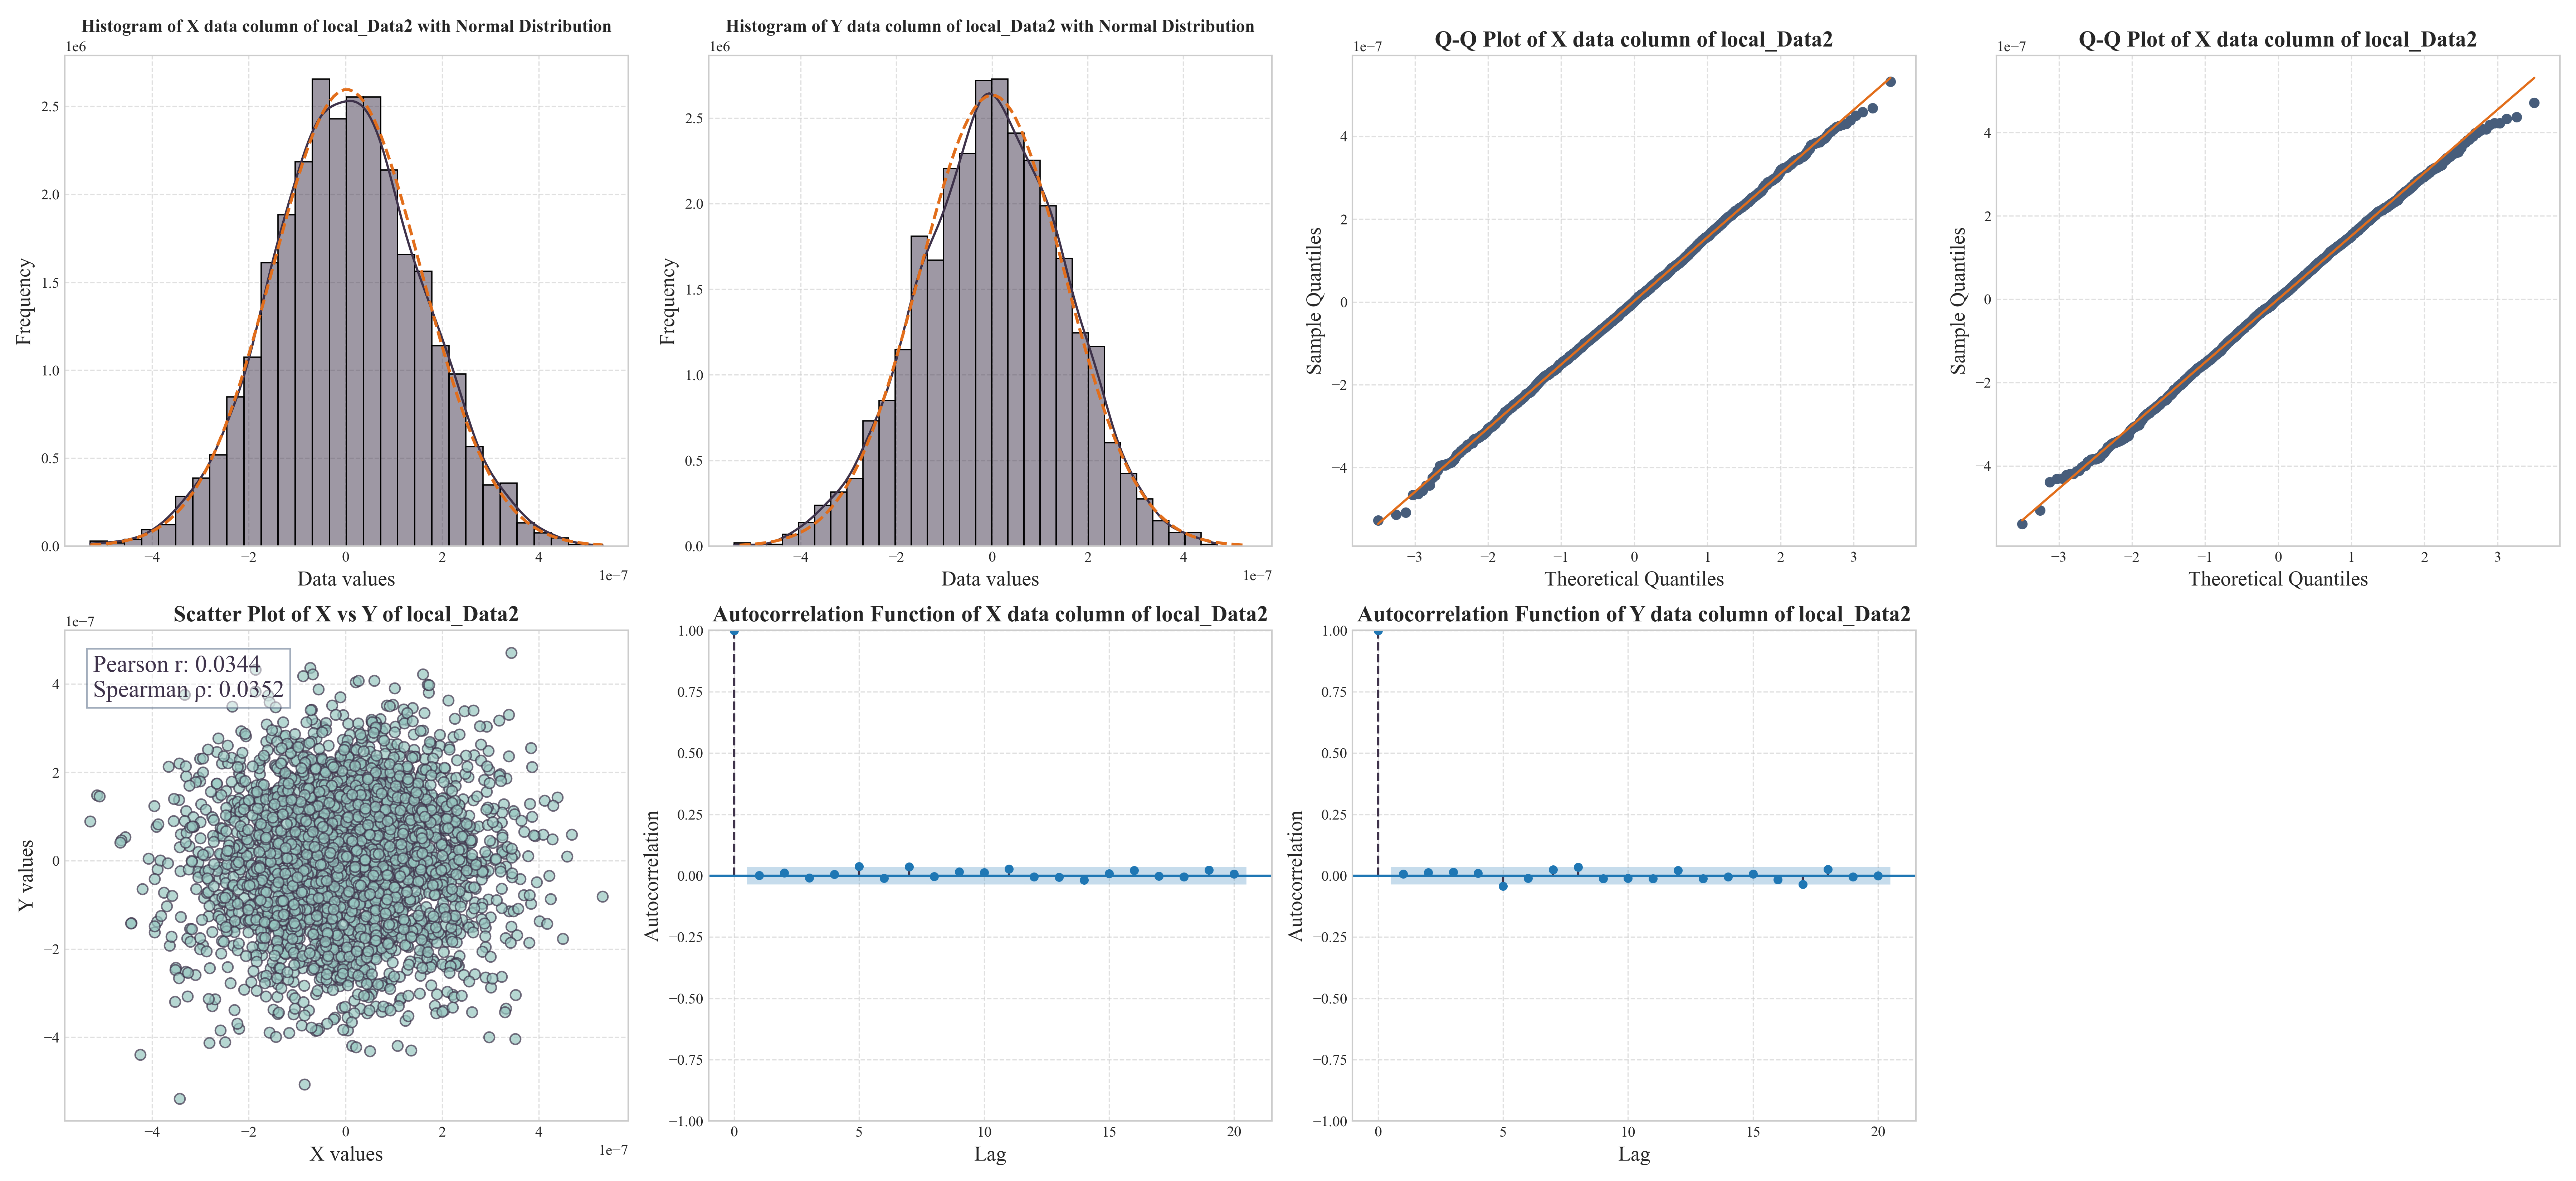
\includegraphics[width=\linewidth]{images/correlation-analysis-output/local_Data2}
			\caption{数据质量评定：现场测量Data2}
			\label{fig:localdata2}
		\end{figure}
		
		\item 对数据 \texttt{local\_Data3} 的 \(X\) 数据列进行正则分布检验，结果如下所示：
		
		\begin{itemize}
			\item \textbf{Shapiro-Wilk 检验}:
			\begin{itemize}
				\item 统计量: \(0.9988\), p 值: \(0.0244\)
				\item 结论: 数据不符合正态分布假设 (p < 0.05)
			\end{itemize}
			
			\item \textbf{Kolmogorov-Smirnov 检验}:
			\begin{itemize}
				\item 统计量: \(0.0085\), p 值: \(0.9703\)
				\item 结论: 数据符合正态分布假设 (p > 0.05)
			\end{itemize}
			
			\item \textbf{简化卡方检验}:
			\begin{itemize}
				\item 简化卡方值: \(180.9434\)
				\item 结论: 数据不符合正态分布假设 (卡方值 < 临界值)
			\end{itemize}
		\end{itemize}
		
		对数据 \texttt{local\_Data3} 的 \(Y\) 数据列进行正则分布检验，结果如下所示：
		
		\begin{itemize}
			\item \textbf{Shapiro-Wilk 检验}:
			\begin{itemize}
				\item 统计量: \(0.9992\), p 值: \(0.1836\)
				\item 结论: 数据符合正态分布假设 (p > 0.05)
			\end{itemize}
			
			\item \textbf{Kolmogorov-Smirnov 检验}:
			\begin{itemize}
				\item 统计量: \(0.0122\), p 值: \(0.7126\)
				\item 结论: 数据符合正态分布假设 (p > 0.05)
			\end{itemize}
			
			\item \textbf{简化卡方检验}:
			\begin{itemize}
				\item 简化卡方值: \(16.3325\)
				\item 结论: 数据符合正态分布假设 (卡方值 < 临界值)
			\end{itemize}
		\end{itemize}
		
		对数据 \texttt{local\_Data3} 进行相关性分析，结果如下所示：
		
		\begin{itemize}
			\item \textbf{Pearson 相关系数}:
			\begin{itemize}
				\item 系数: \(0.0265\), p 值: \(0.1310\)
				\item 结论: 在显著性水平 0.05 下，两列数据不存在显著的线性相关性 (p > 0.05)
			\end{itemize}
			
			\item \textbf{Spearman 相关系数}:
			\begin{itemize}
				\item 系数: \(0.0162\), p 值: \(0.3574\)
				\item 结论: 在显著性水平 0.05 下，两列数据不存在显著的非参数相关性 (p > 0.05)
			\end{itemize}
		\end{itemize}
		
		\begin{figure}[h!]
			\centering
			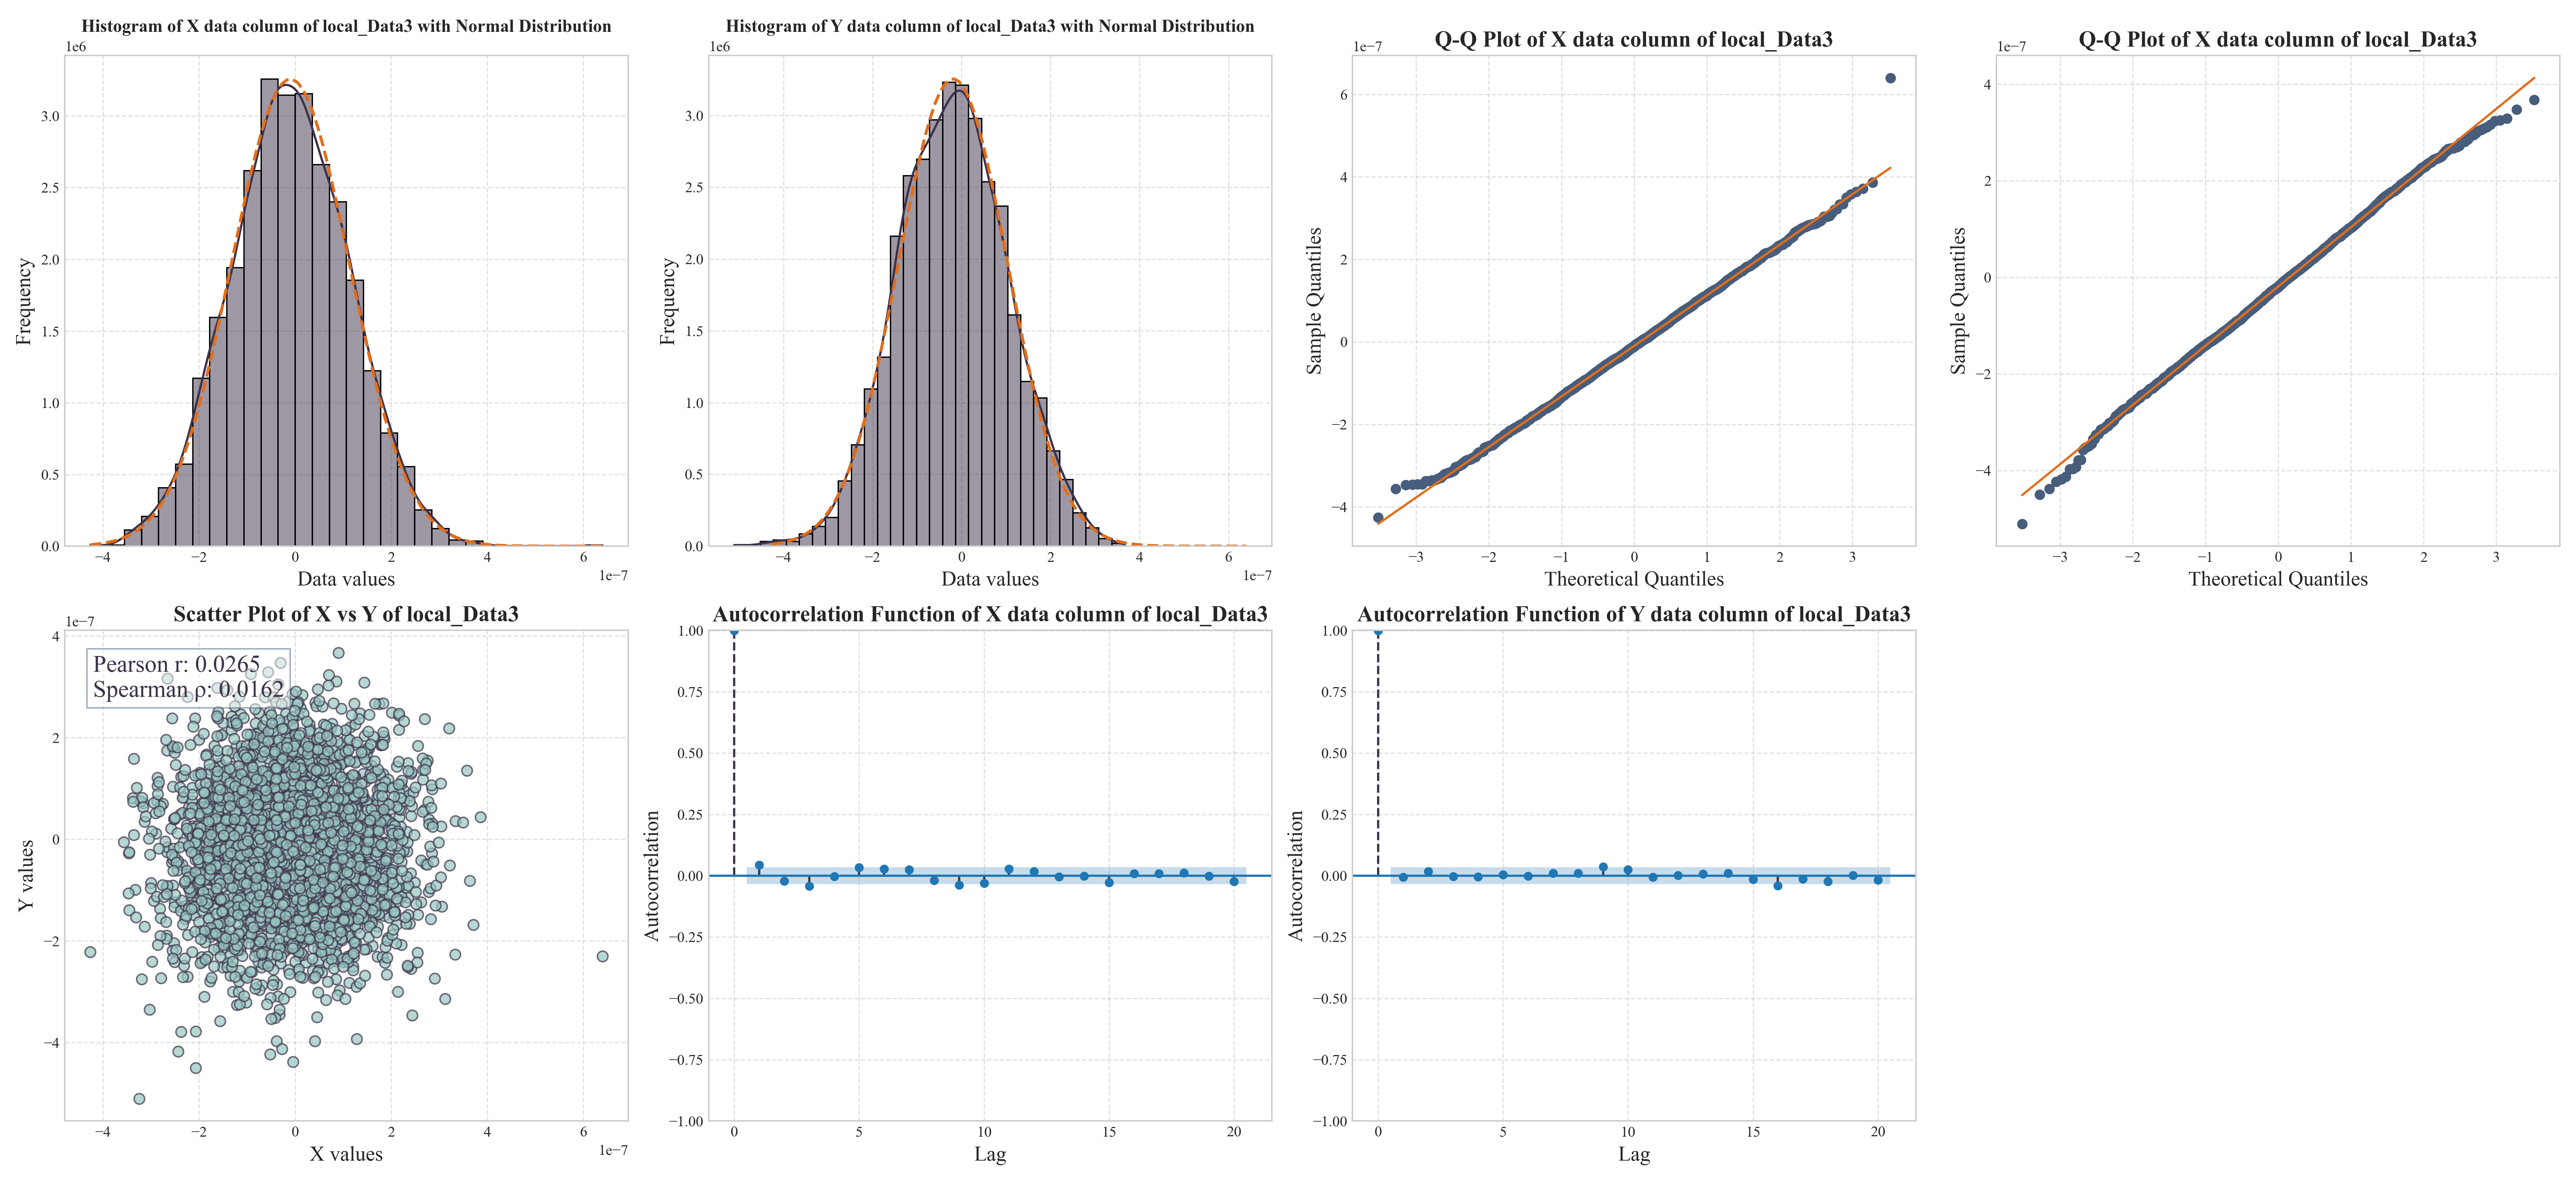
\includegraphics[width=\linewidth]{images/correlation-analysis-output/local_Data3}
			\caption{数据质量评定：现场测量Data3}
			\label{fig:localdata3}
		\end{figure}
		
		\item 对数据 \texttt{remote\_Data4} 的 \(X\) 数据列进行正则分布检验，结果如下所示：
		
		\begin{itemize}
			\item \textbf{Shapiro-Wilk 检验}:
			\begin{itemize}
				\item 统计量: \(0.9981\), p 值: \(0.0860\)
				\item 结论: 数据符合正态分布假设 (p > 0.05)
			\end{itemize}
			
			\item \textbf{Kolmogorov-Smirnov 检验}:
			\begin{itemize}
				\item 统计量: \(0.0171\), p 值: \(0.7705\)
				\item 结论: 数据符合正态分布假设 (p > 0.05)
			\end{itemize}
			
			\item \textbf{简化卡方检验}:
			\begin{itemize}
				\item 简化卡方值: \(18.8169\)
				\item 结论: 数据不符合正态分布假设 (卡方值 > 临界值)
			\end{itemize}
		\end{itemize}
		
		对数据 \texttt{remote\_Data4} 的 \(Y\) 数据列进行正则分布检验，结果如下所示：
		
		\begin{itemize}
			\item \textbf{Shapiro-Wilk 检验}:
			\begin{itemize}
				\item 统计量: \(0.9991\), p 值: \(0.7438\)
				\item 结论: 数据符合正态分布假设 (p > 0.05)
			\end{itemize}
			
			\item \textbf{Kolmogorov-Smirnov 检验}:
			\begin{itemize}
				\item 统计量: \(0.0122\), p 值: \(0.9786\)
				\item 结论: 数据符合正态分布假设 (p > 0.05)
			\end{itemize}
			
			\item \textbf{简化卡方检验}:
			\begin{itemize}
				\item 简化卡方值: \(8.5004\)
				\item 结论: 数据符合正态分布假设 (卡方值 < 临界值)
			\end{itemize}
		\end{itemize}
		
		对数据 \texttt{remote\_Data4} 进行相关性分析，结果如下所示：
		
		\begin{itemize}
			\item \textbf{Pearson 相关系数}:
			\begin{itemize}
				\item 系数: \(0.0396\), p 值: \(0.1282\)
				\item 结论: 在显著性水平 0.05 下，两列数据不存在显著的线性相关性 (p > 0.05)
			\end{itemize}
			
			\item \textbf{Spearman 相关系数}:
			\begin{itemize}
				\item 系数: \(0.0413\), p 值: \(0.1123\)
				\item 结论: 在显著性水平 0.05 下，两列数据不存在显著的非参数相关性 (p > 0.05)
			\end{itemize}
		\end{itemize}
		
		\begin{figure}[h!]
			\centering
			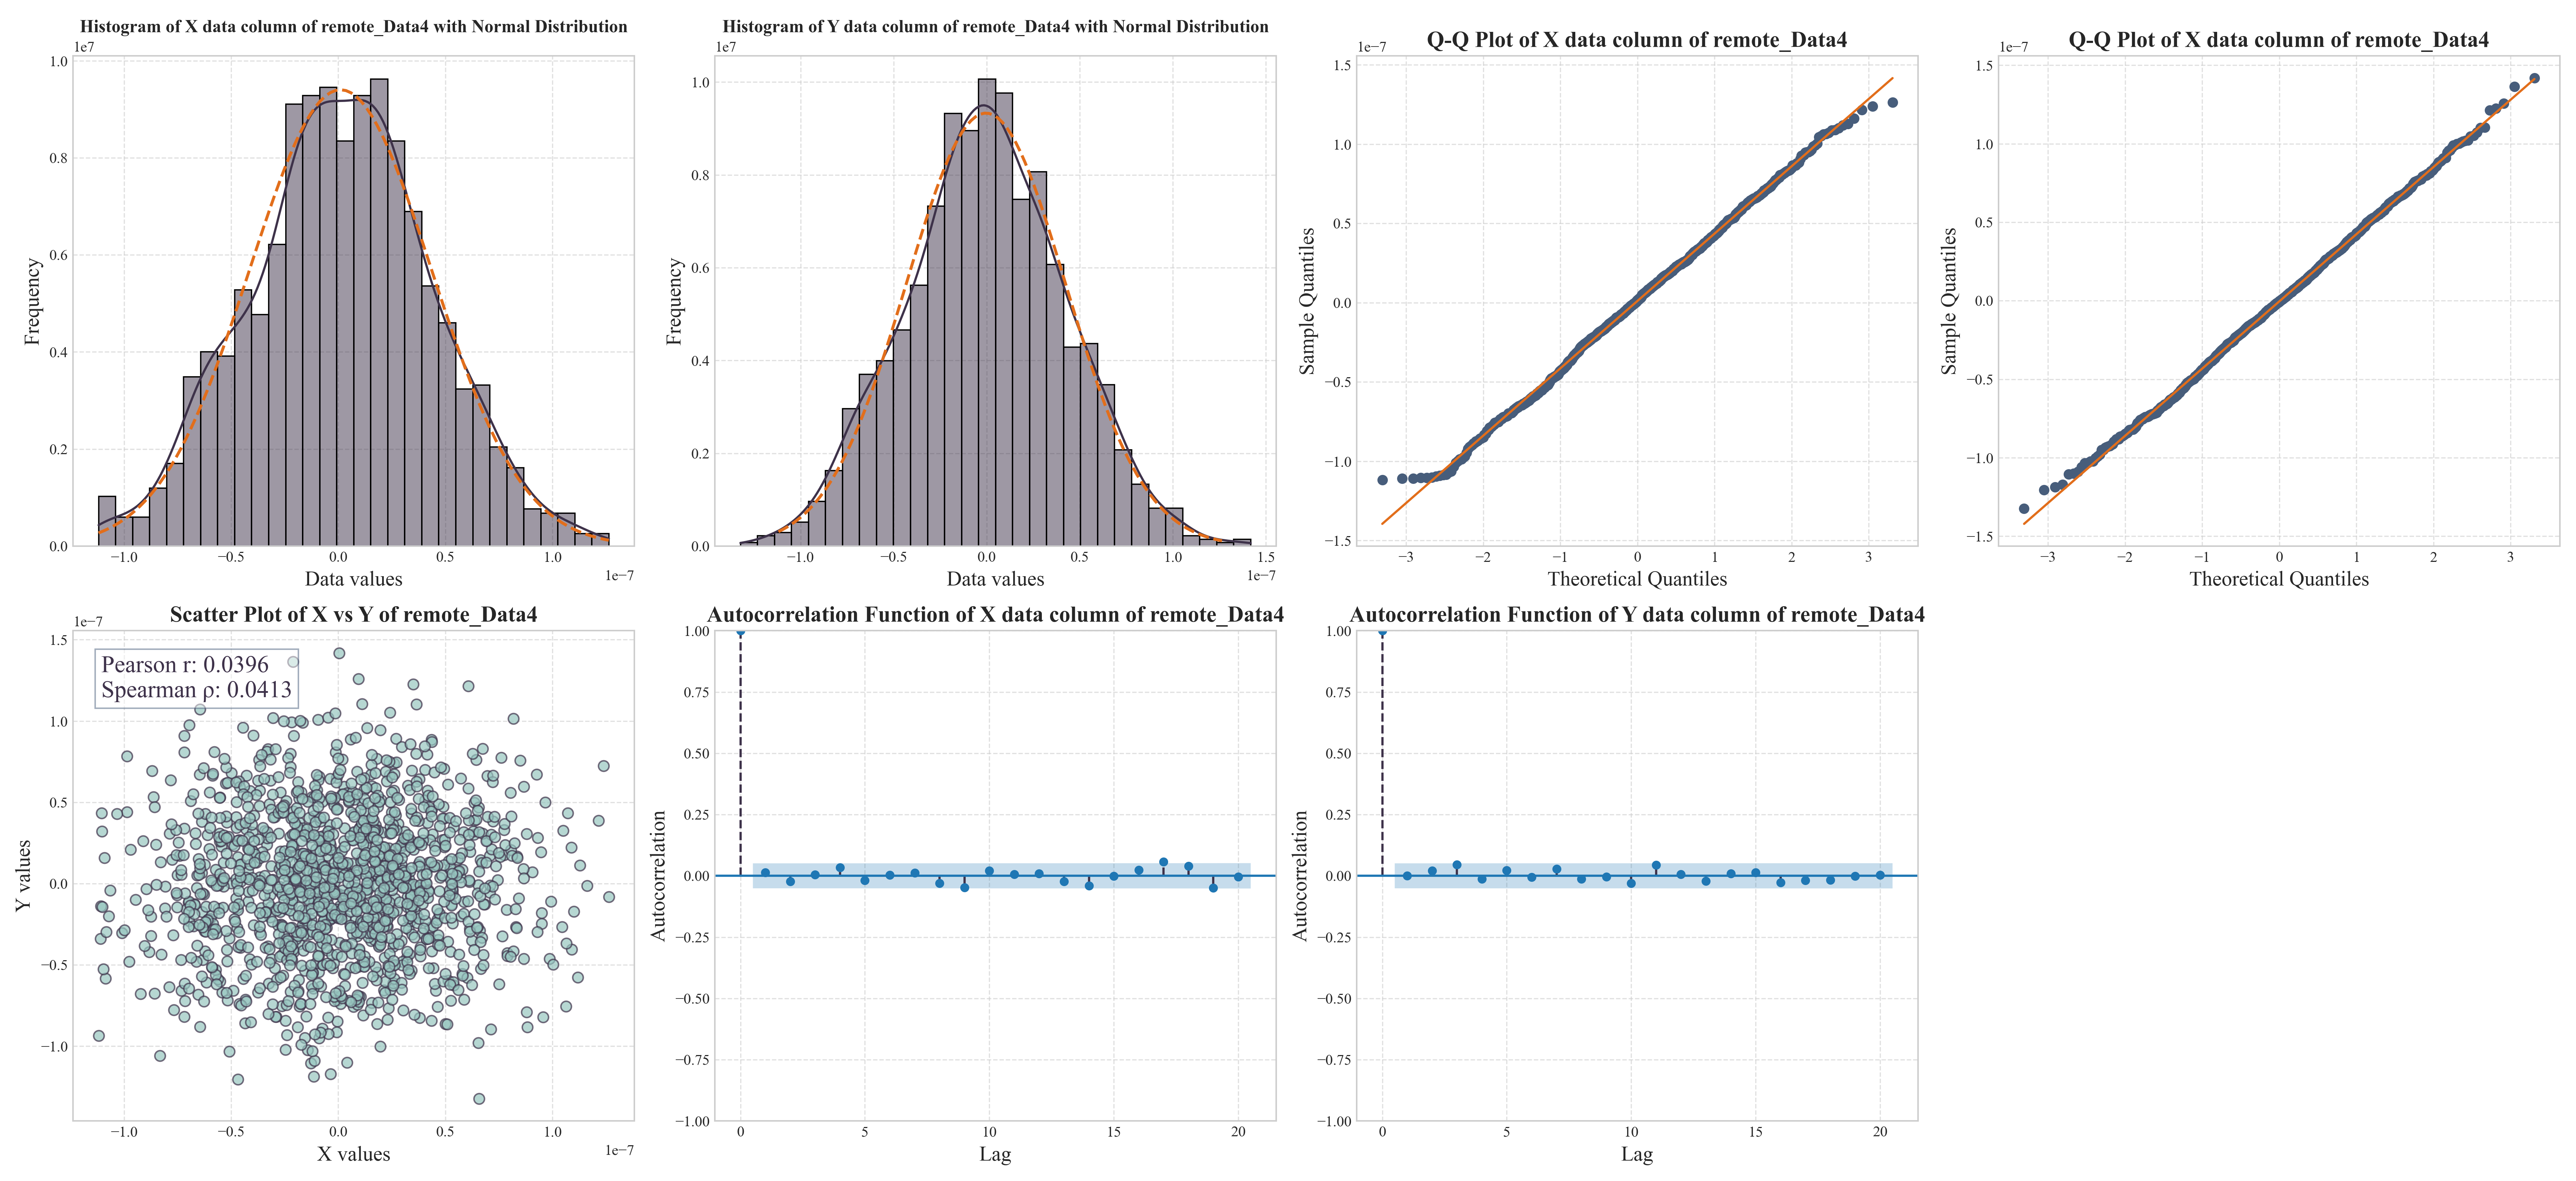
\includegraphics[width=\linewidth]{images/correlation-analysis-output/remote_Data4}
			\caption{数据质量评定：远程测量Data4}
			\label{fig:remotedata4}
		\end{figure}
		
		对数据 \texttt{remote\_Data9} 的 \(X\) 数据列进行正则分布检验，结果如下所示：
		
		\begin{itemize}
			\item \textbf{Shapiro-Wilk 检验}:
			\begin{itemize}
				\item 统计量: \(0.9986\), p 值: \(0.4378\)
				\item 结论: 数据符合正态分布假设 (p > 0.05)
			\end{itemize}
			
			\item \textbf{Kolmogorov-Smirnov 检验}:
			\begin{itemize}
				\item 统计量: \(0.0194\), p 值: \(0.7260\)
				\item 结论: 数据符合正态分布假设 (p > 0.05)
			\end{itemize}
			
			\item \textbf{简化卡方检验}:
			\begin{itemize}
				\item 简化卡方值: \(11.3080\)
				\item 结论: 数据符合正态分布假设 (卡方值 < 临界值)
			\end{itemize}
		\end{itemize}
		
		对数据 \texttt{remote\_Data9} 的 \(Y\) 数据列进行正则分布检验，结果如下所示：
		
		\begin{itemize}
			\item \textbf{Shapiro-Wilk 检验}:
			\begin{itemize}
				\item 统计量: \(0.9983\), p 值: \(0.2221\)
				\item 结论: 数据符合正态分布假设 (p > 0.05)
			\end{itemize}
			
			\item \textbf{Kolmogorov-Smirnov 检验}:
			\begin{itemize}
				\item 统计量: \(0.0240\), p 值: \(0.4590\)
				\item 结论: 数据符合正态分布假设 (p > 0.05)
			\end{itemize}
			
			\item \textbf{简化卡方检验}:
			\begin{itemize}
				\item 简化卡方值: \(23.7076\)
				\item 结论: 数据不符合正态分布假设 (卡方值 > 临界值)
			\end{itemize}
		\end{itemize}
		
		对数据 \texttt{remote\_Data9} 进行相关性分析，结果如下所示：
		
		\begin{itemize}
			\item \textbf{Pearson 相关系数}:
			\begin{itemize}
				\item 系数: \(0.0195\), p 值: \(0.4903\)
				\item 结论: 在显著性水平 0.05 下，两列数据不存在显著的线性相关性 (p > 0.05)
			\end{itemize}
			
			\item \textbf{Spearman 相关系数}:
			\begin{itemize}
				\item 系数: \(0.0113\), p 值: \(0.6883\)
				\item 结论: 在显著性水平 0.05 下，两列数据不存在显著的非参数相关性 (p > 0.05)
			\end{itemize}
		\end{itemize}
		
		\begin{figure}[h!]
			\centering
			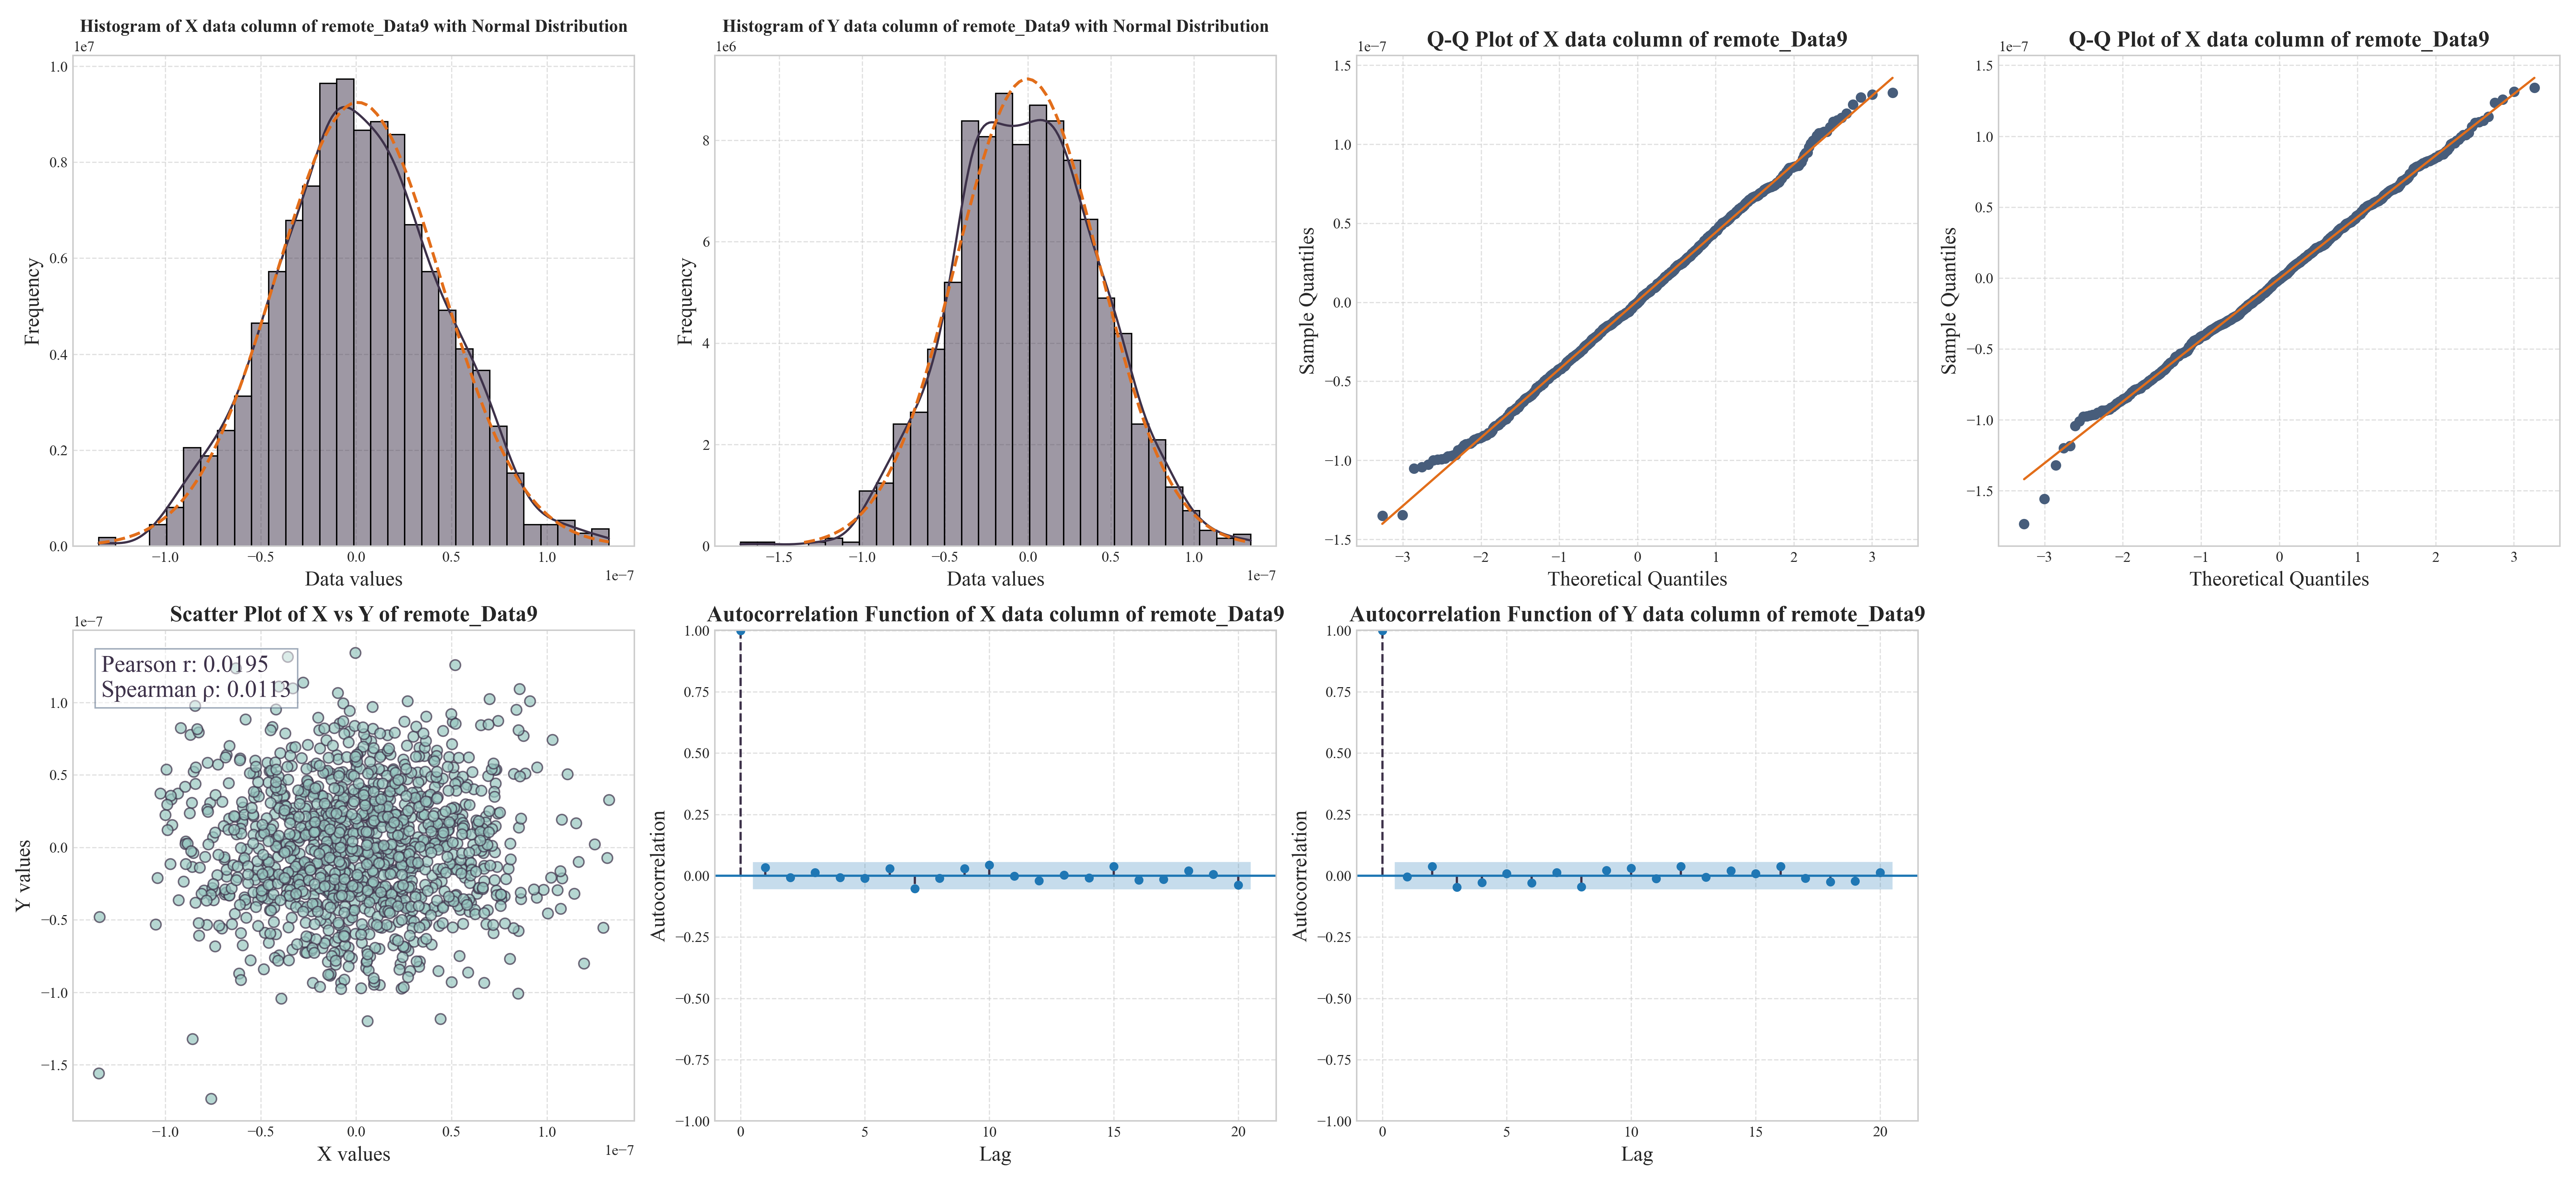
\includegraphics[width=\linewidth]{images/correlation-analysis-output/remote_Data9}
			\caption{数据质量评定：远程测量Data9}
			\label{fig:remotedata9}
		\end{figure}
		
	\end{enumerate}
	
	\item 计算玻尔兹曼常数
	
	通过计算噪声强度，对电阻热噪声测量值的输入带宽修正、扣除本底和噪声功率谱密度计算最终实现玻尔兹曼常量计算（计算代码见\textbf{附件}）。结果如\cref{tab:kbvalues}所示。
	
	\begin{table}[h!]
		\centering
		\renewcommand{\arraystretch}{1.5} % 调整行高
		\caption{本地测量与遥测测量的 $k_B$ 值（单位：J/K）}
		\label{tab:kbvalues}
		\begin{tabular}{|cc|cc|}
			\hline
			\textbf{数据名} & \textbf{本地测量列 $k_B$ (local)} & \textbf{数据名} & \textbf{遥测测量列 $k_B$ (remote)} \\ \hline
			local/Data1 & $1.12\times10^{-23}$ & remote/Data2 & $1.72\times10^{-23}$ \\ 
			local/Data2 & $1.42\times10^{-23}$ & remote/Data3 & $1.35\times10^{-23}$ \\ 
			local/Data3 & $1.38\times10^{-23}$ & remote/Data4 & $1.35\times10^{-23}$ \\ 
			local/Data4 & $1.43\times10^{-23}$ & remote/Data5 & $1.43\times10^{-23}$ \\ 
			local/Data5 & $7.65\times10^{-24}$ & remote/Data6 & $1.35\times10^{-23}$ \\ 
			local/Data6 & $1.47\times10^{-23}$ & remote/Data7 & $1.88\times10^{-23}$ \\ 
			local/Data7 & $2.61\times10^{-23}$ & remote/Data8 & $1.62\times10^{-23}$ \\ 
			local/Data8 & $1.70\times10^{-23}$ & remote/Data9 & $1.42\times10^{-23}$ \\ \hline
		\end{tabular}
	\end{table}
	
	本地测量均值：	$1.48\times10^{-23}$J/K；
	
	\begin{figure}[h!]
		\centering
		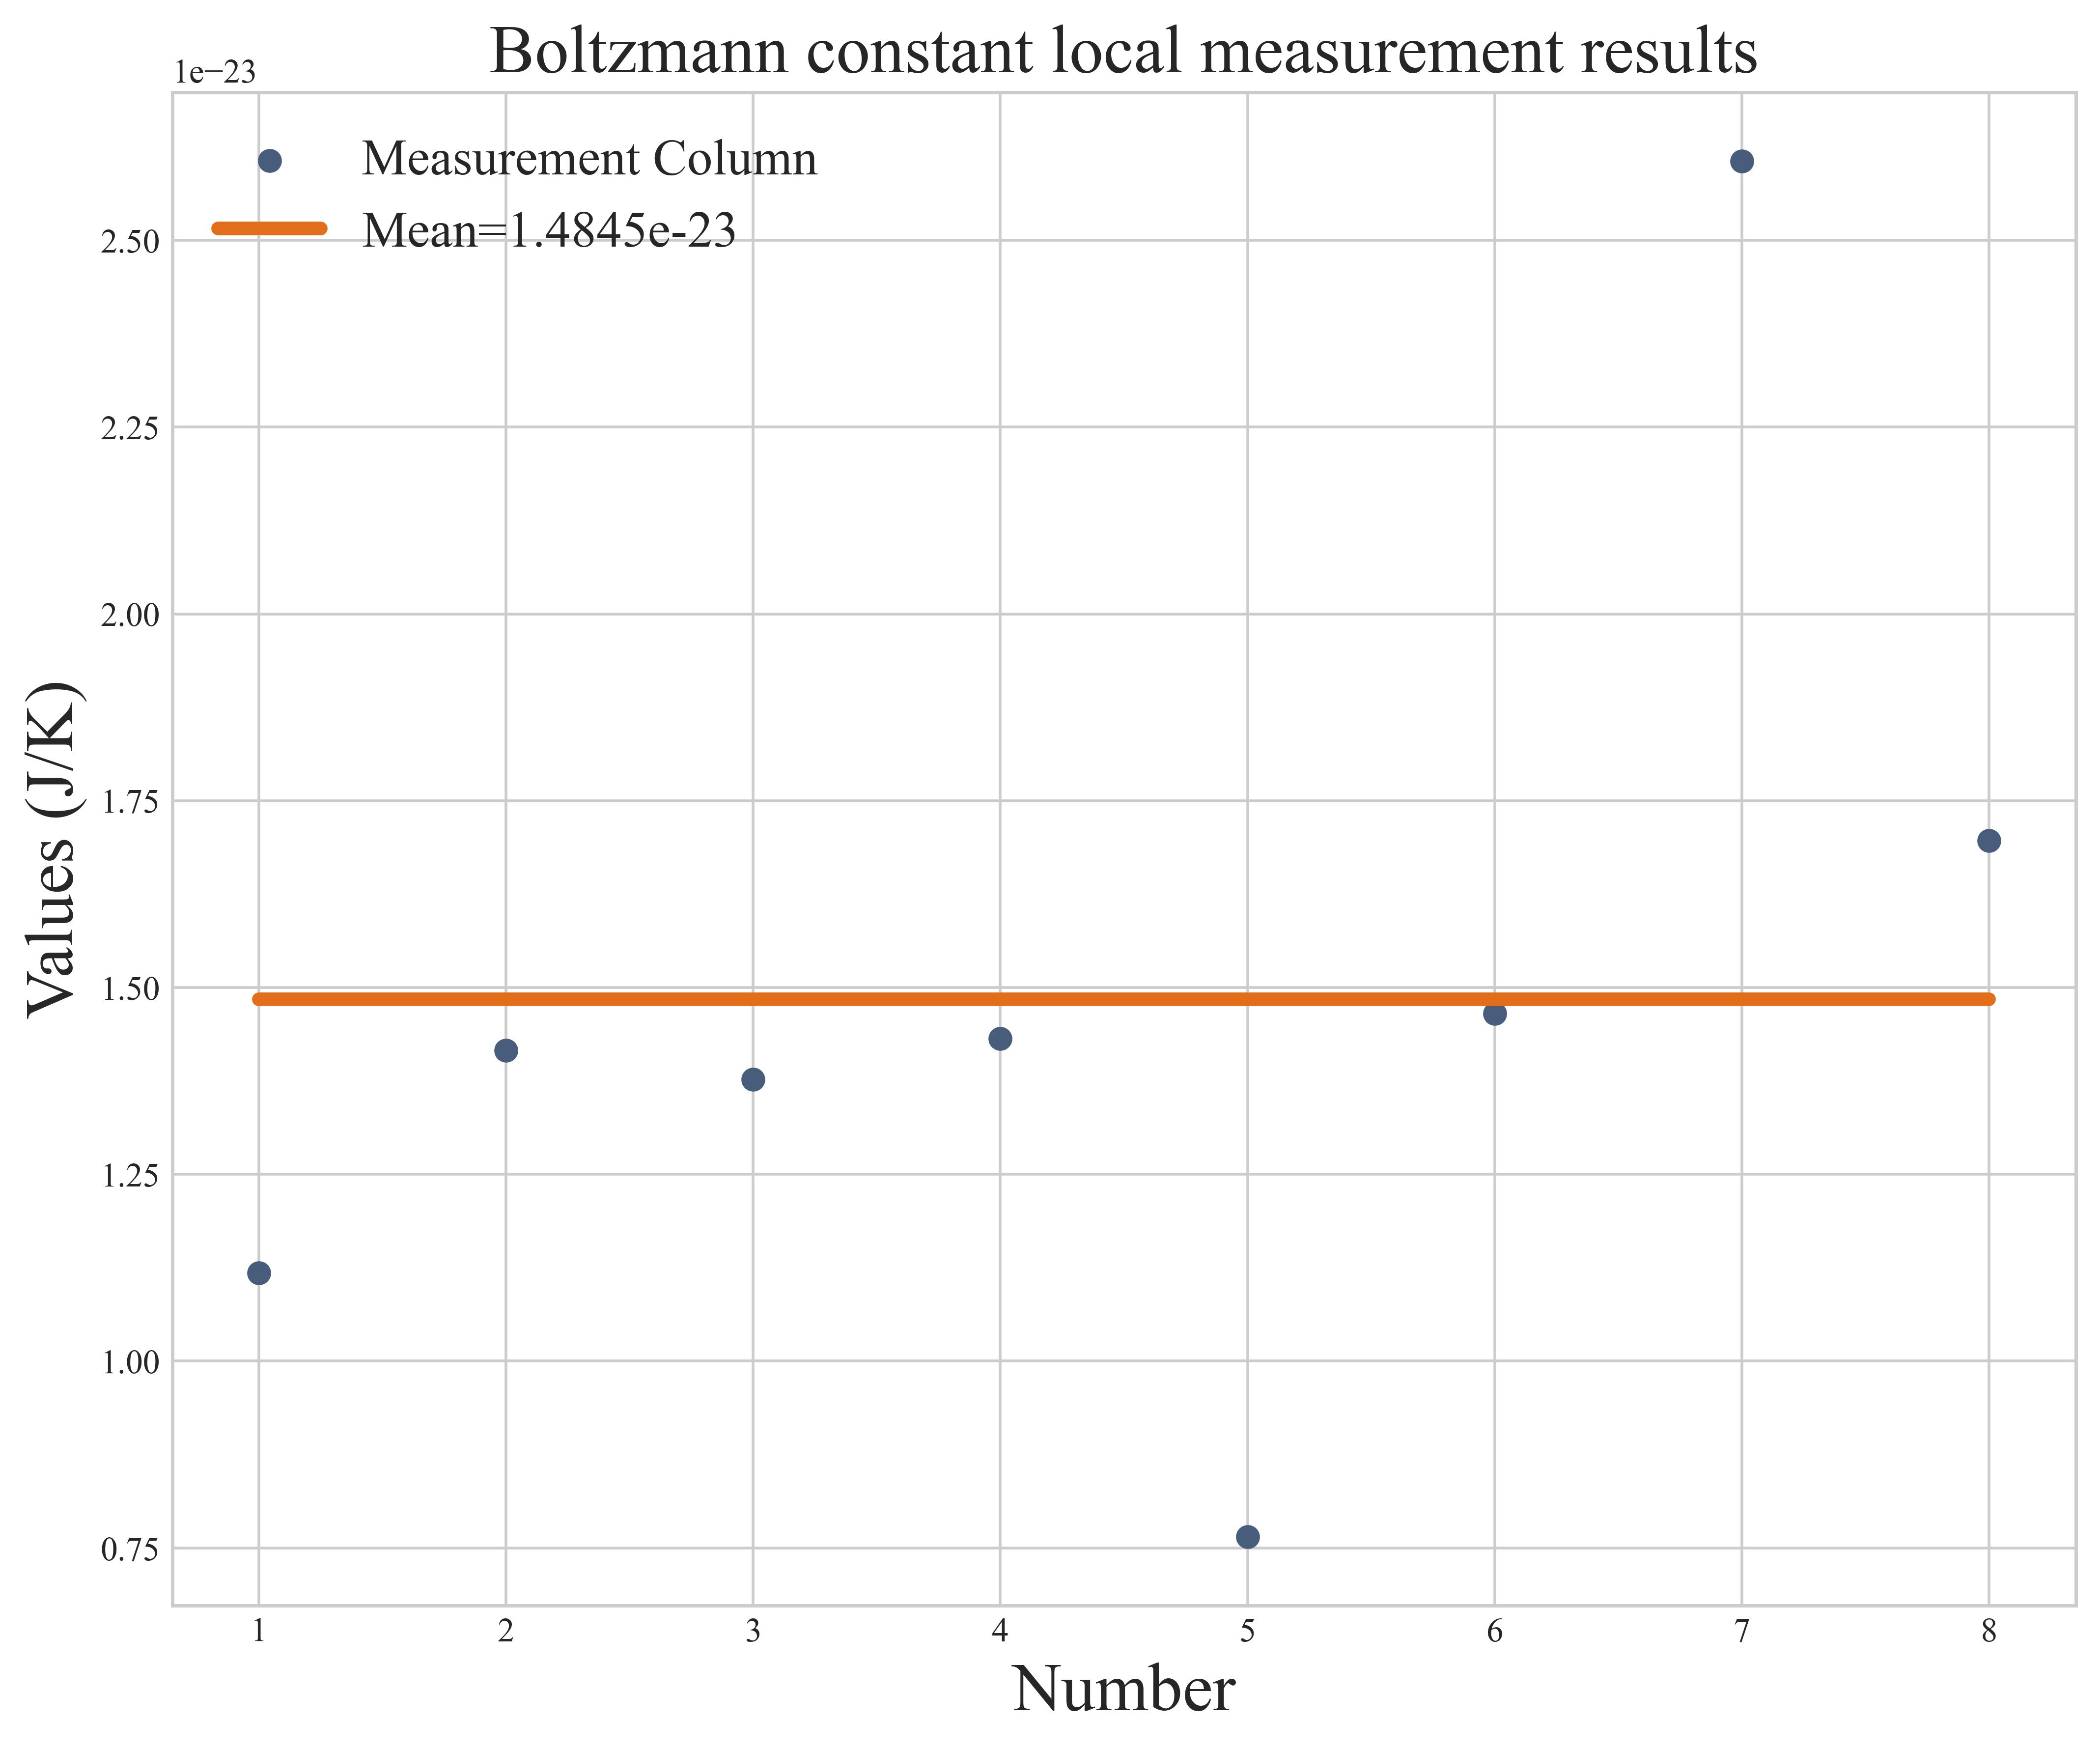
\includegraphics[width=0.5\linewidth]{images/APL1_1_A_kB_local}
		\caption{本地测量均值}
		\label{fig:apl11akblocal}
	\end{figure}
	
	遥测均值：$1.51\times10^{-23}$J/K。
	
	\begin{figure}[h!]
		\centering
		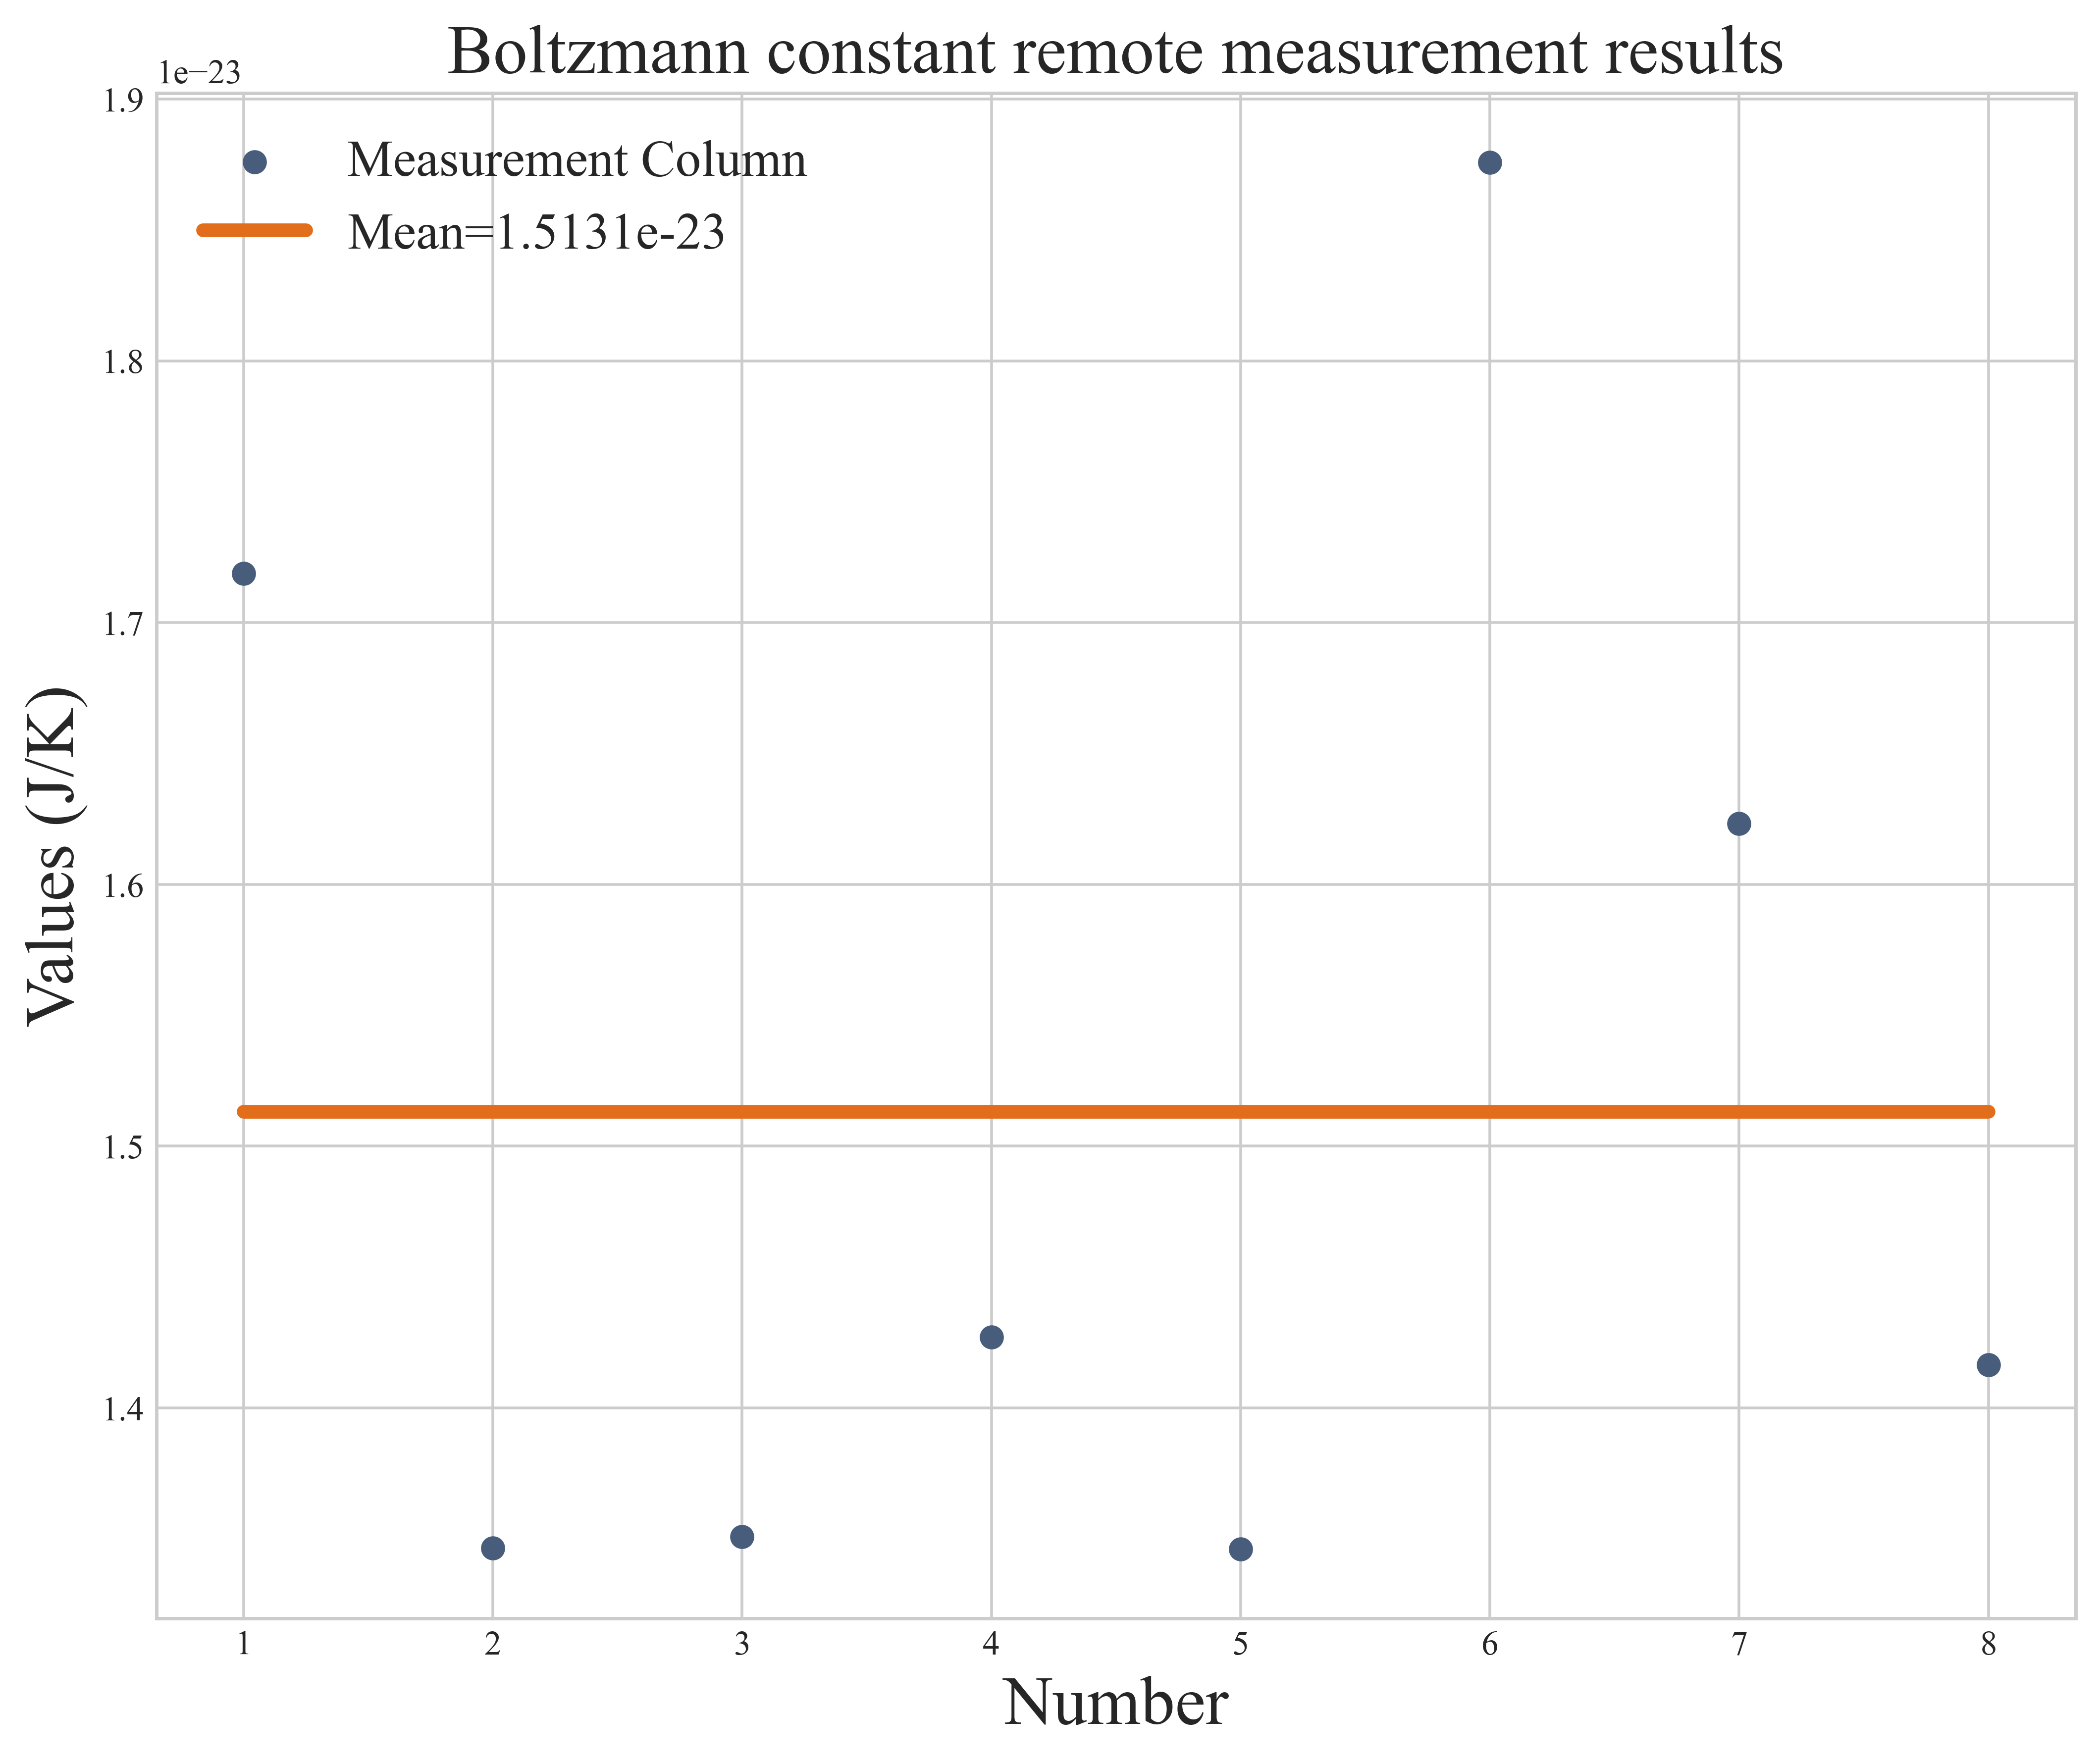
\includegraphics[width=0.5\linewidth]{images/APL1_1_A_kB_remote}
		\caption{遥测均值}
		\label{fig:apl11akbremote}
	\end{figure}
	
	从图\cref{fig:apl11akblocal}和\cref{fig:apl11akbremote}可以看出，数据的离散程度还是较大的，具体见\textbf{误差分析}部分。
	
	\item 误差分析
	
	这里参考\cite{g}和\cite{c}中内容提出误差分析的方案。
	
	首先根据\cite{g}，假设\textbf{锁相放大器的数值低通滤波器的相对误差可以忽略不计}，电阻 $R$，温度 $T$ 独立测量，其\textbf{误差主要取决于测量仪器的系统误差}。由误差传递可得 $k_B$ 的比值不确定度为：
	\[
	\frac{\delta k_B}{k_B} = \frac{1}{4} \left(\sqrt{\left( 1 + 2 \frac{n_{Bx}^2}{n_{Tx}^2} \right) \frac{8}{M - 1} + \frac{\delta R}{R} + \frac{\delta T}{T}}\right)
	\]
	
	接下来，\cite{c}对上述误差作了进一步讨论，它采用了基于\cite{g}的“保守估计”，取热噪声测量 3 倍标准差 $3\sigma_{n_{TX}}$ (置信度 99.7\%) 计算玻尔兹曼常量测量的最大不确定度为：
	\[
	\frac{\delta k_B}{k_B} = 3\sqrt{\left(1 + 2\frac{n_{BX}^2}{n_{TX}^2}\right)\frac{2}{M-1} + \left|\frac{\delta R}{R}\right| + \left|\frac{\delta T}{T}\right| + 2\frac{\delta \alpha}{\alpha}}
	\]
	其中，电阻与温度的测量随机误差远小于 1\%，可忽略。
	这里只考虑系统误差：设手持多用表测量电阻最大不确定度 $\delta R = 1 \, \Omega$，测温仪在室温和液氮下测温最大不确定度 $\delta T$ 为 0.3 K 和 2 K；
	OE1022 手册中给出的 $\delta \alpha/\alpha \leq 1\%$，标准为 2\%。
	
	此外，它还提到了输入带宽修正也会给测量电压带来比值不确定度 $\delta v_{\text{BW}} / v_{\text{BW}}$，具体表示为
	\[
	\frac{\delta v_{\text{BW}}}{v_{\text{BW}}} = 
	\left( 1 + \frac{n_{BX}^2}{n_{TX}^2} \right)
	\frac{ \left( \omega R_{\text{in}} C_{\text{in}} \right)^2 }{ 1 + \left( \omega R_{\text{in}} C_{\text{in}} \right)^2 }
	\left( \frac{\delta R_{\text{in}}}{R_{\text{in}}} + \frac{\delta C_{\text{in}}}{C_{\text{in}}} \right)
	\]
	
	最后，两篇文献中都提到了现场测量的误差比遥测更大，例如\cref{fig:apl11aenvnoise}所示。
	
	\begin{figure}[h!]
		\centering
		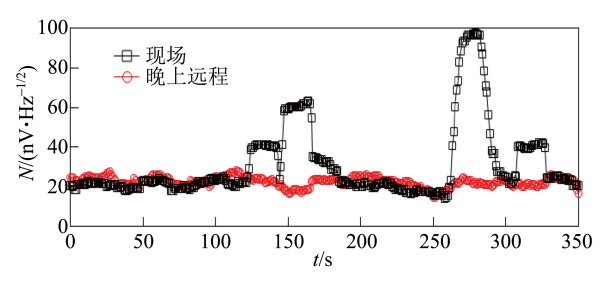
\includegraphics[width=0.5\linewidth]{images/APL1_1_A_env_noise}
		\caption{环境噪声的影响（来自\cite{c}）}
		\label{fig:apl11aenvnoise}
	\end{figure}。
	
	事实上，我们考虑一方面还需查找更多资料做更完善更全面的误差分析；另一方面我们需要结合实验结果进行具体的误差分析。
	
	\begin{ubox}{}
		遗憾的是，上述误差分析方案并不是一个良好的方案，它只给出了相对误差的最大估计，采用该方案分析我们的实验数据得到的最大误差超过60\%，因此我们需要一个更准确的计算方案。
		
		利用误差传递公式，我们给出以下估计，一个$\sigma$以内：
		$$
		\frac{\delta k_B}{k_B} = \sqrt{\left(1 + 2\frac{n_{BX}^2}{n_{TX}^2}\right)\frac{2}{M-1} + \left|\frac{\delta R}{R^3}\right|^2 + \left|\frac{\delta T}{T^3}\right|^2 + 2(\frac{\delta \alpha}{\alpha})^2}
		$$
		
		而在置信度99.7\%的3$\sigma$范围内，估计如下：
		$$
		\frac{\delta k_B}{k_B} = 3\sqrt{\left(1 + 2\frac{n_{BX}^2}{n_{TX}^2}\right)\frac{2}{M-1} + \left|\frac{\delta R}{R^3}\right|^2 + \left|\frac{\delta T}{T^3}\right|^2 + 2(\frac{\delta \alpha}{\alpha})^2}
		$$
		
		按此计算（相关数据处理代码见\textbf{附件}）得到结果如\cref{tab:relative_error}所示。
		
	\end{ubox}
	
	\begin{table}[h!]
		\centering
		\renewcommand{\arraystretch}{1.5} % 调整行高
		\caption{相对误差数据表}
		\label{tab:relative_error}
		\begin{tabular}{|ccccc|}
			\hline
			\textbf{数据名} & \textbf{local/Data1} & \textbf{local/Data2} & \textbf{local/Data3} & \textbf{local/Data4}  \\ 
			\textbf{相对误差（本地测量）} & 9.90\% & 9.94\% & 9.67\% & 13.72\% \\ 
			\hline
			\textbf{数据名} & \textbf{local/Data5} & \textbf{local/Data6} & \textbf{local/Data7} & \textbf{local/Data8} \\
			\textbf{相对误差（本地测量）}& 16.91\% & 11.20\% & 15.99\% & 11.80\% \\
			\hline
		\end{tabular}
	\end{table}
	
\end{enumerate}

% 讨论
\subsubsection{Discussion}
本小节展示实验方案预期的\textbf{实验结果讨论}。
\begin{enumerate}
	\item 对 A-B 差分输入做输入带宽修正，其等效输入电阻、电容怎么取？
	
	\begin{figure}[h!]
		\centering
		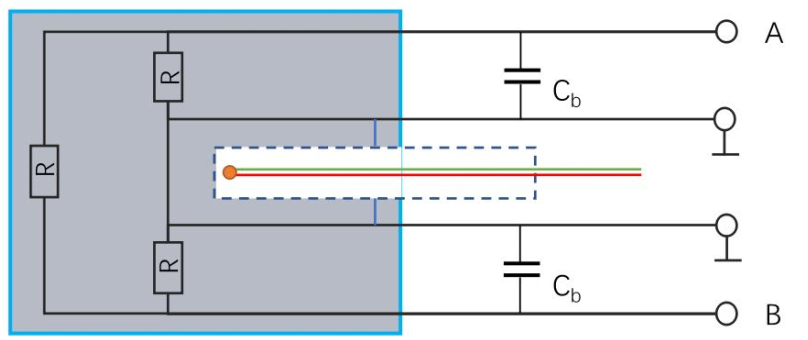
\includegraphics[width=0.5\linewidth]{images/APL1_1_A_RinCin}
		\caption{等效输入电阻、电容示意图}
		\label{fig:apl11arincin}
	\end{figure}
	
	如\cref{fig:apl11arincin}所示，按前述\textbf{原理概述}部分所写，影响输入带宽的 $R_{\text{in}}$ 约为 $2/3R$，$C_{\text{in}}$ 约为电缆电容（室温下约为 96pF/m）、锁相放大器输入电容（25pF），与包括连接器和样品盒在内的电容并联后的值的 1/2（约 \textbf{68pF}）。
	
	\item 经输入带宽修正后的噪声谱密度是否符合热噪声的频谱特征（与频率无关） ？
	
	理论上讲，按原理概述部分\cref{fig:johnson-nyquist-noise-power-spectral-density-of-ideal-resistor}，它应该与频率无关。
	
	但是，将我们的实验测量结果与频率的关系绘制出后，可以明显发现二者是有关系的，最明显的是50000Hz以上，测量值相对于参考值（以及其它测量值）显著偏大，我们合理的怀疑这是一种系统性误差，如\cref{fig:apl11akbflocal}和\cref{fig:apl11akbfremote}所示。
	
	\begin{figure}[h!]
		\centering
		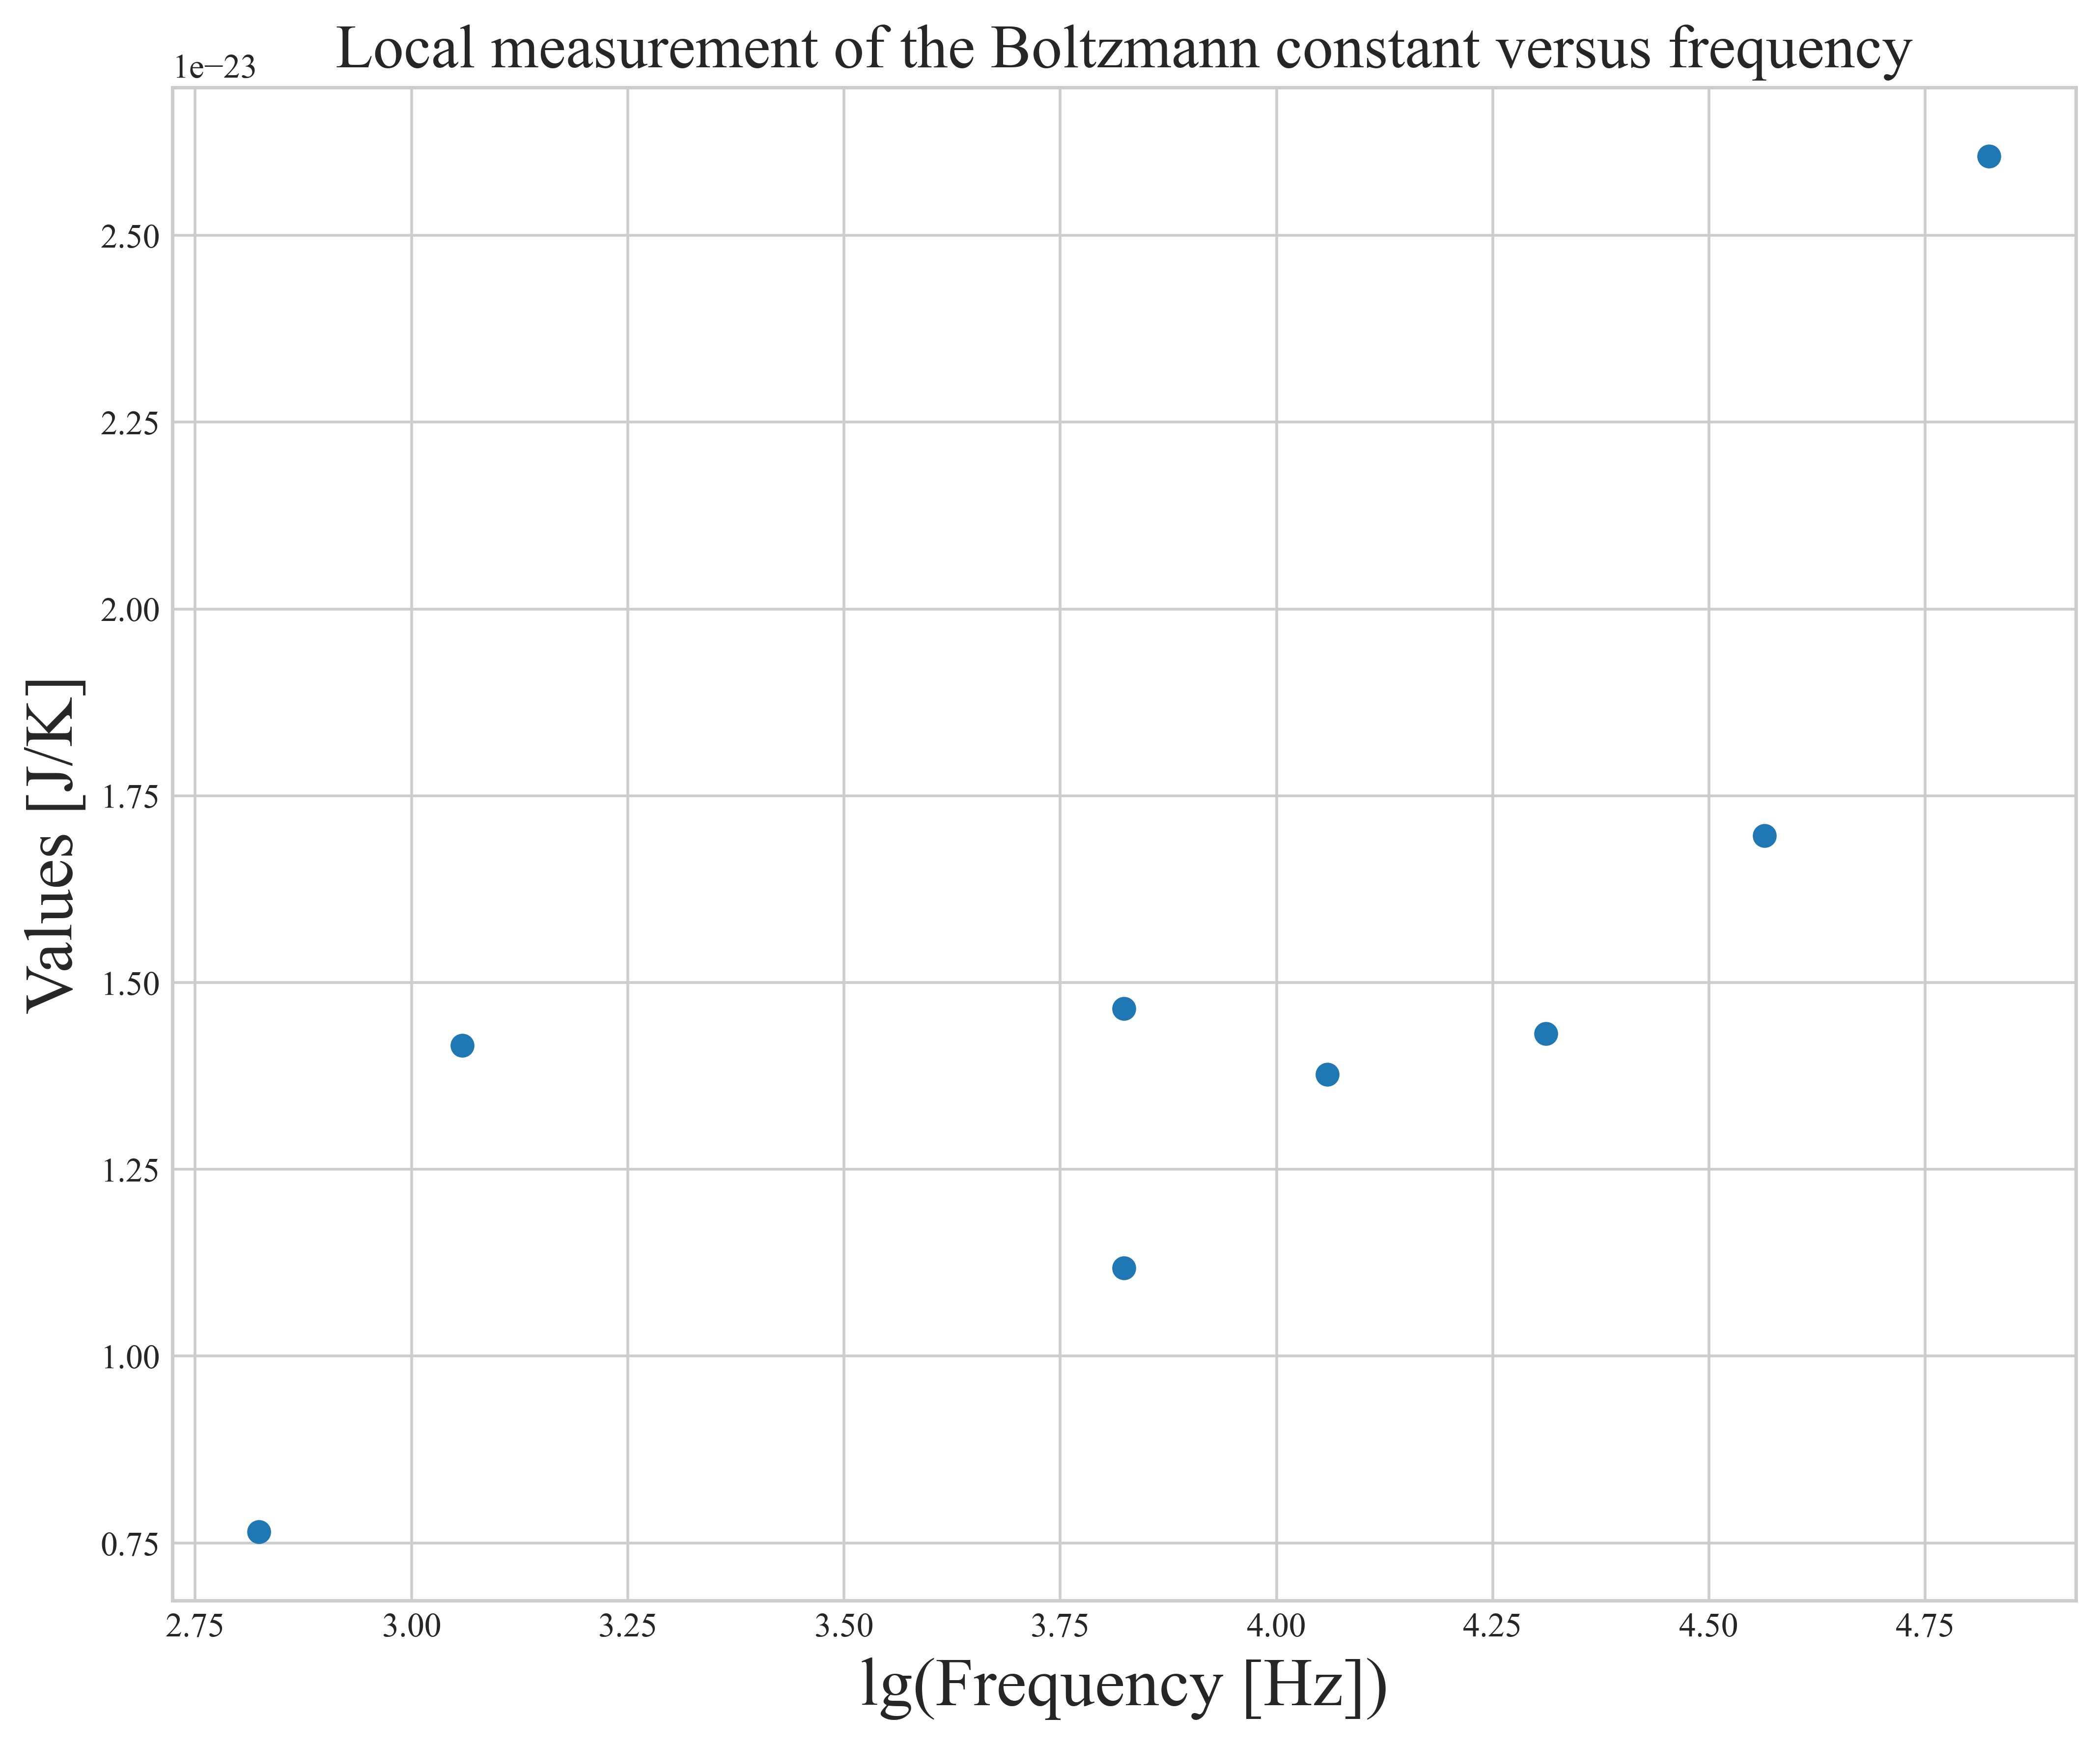
\includegraphics[width=0.7\linewidth]{images/APL1_1_A_kBf_local}
		\caption{本地测量结果的频率分布}
		\label{fig:apl11akbflocal}
	\end{figure}
	
	\begin{figure}[h!]
		\centering
		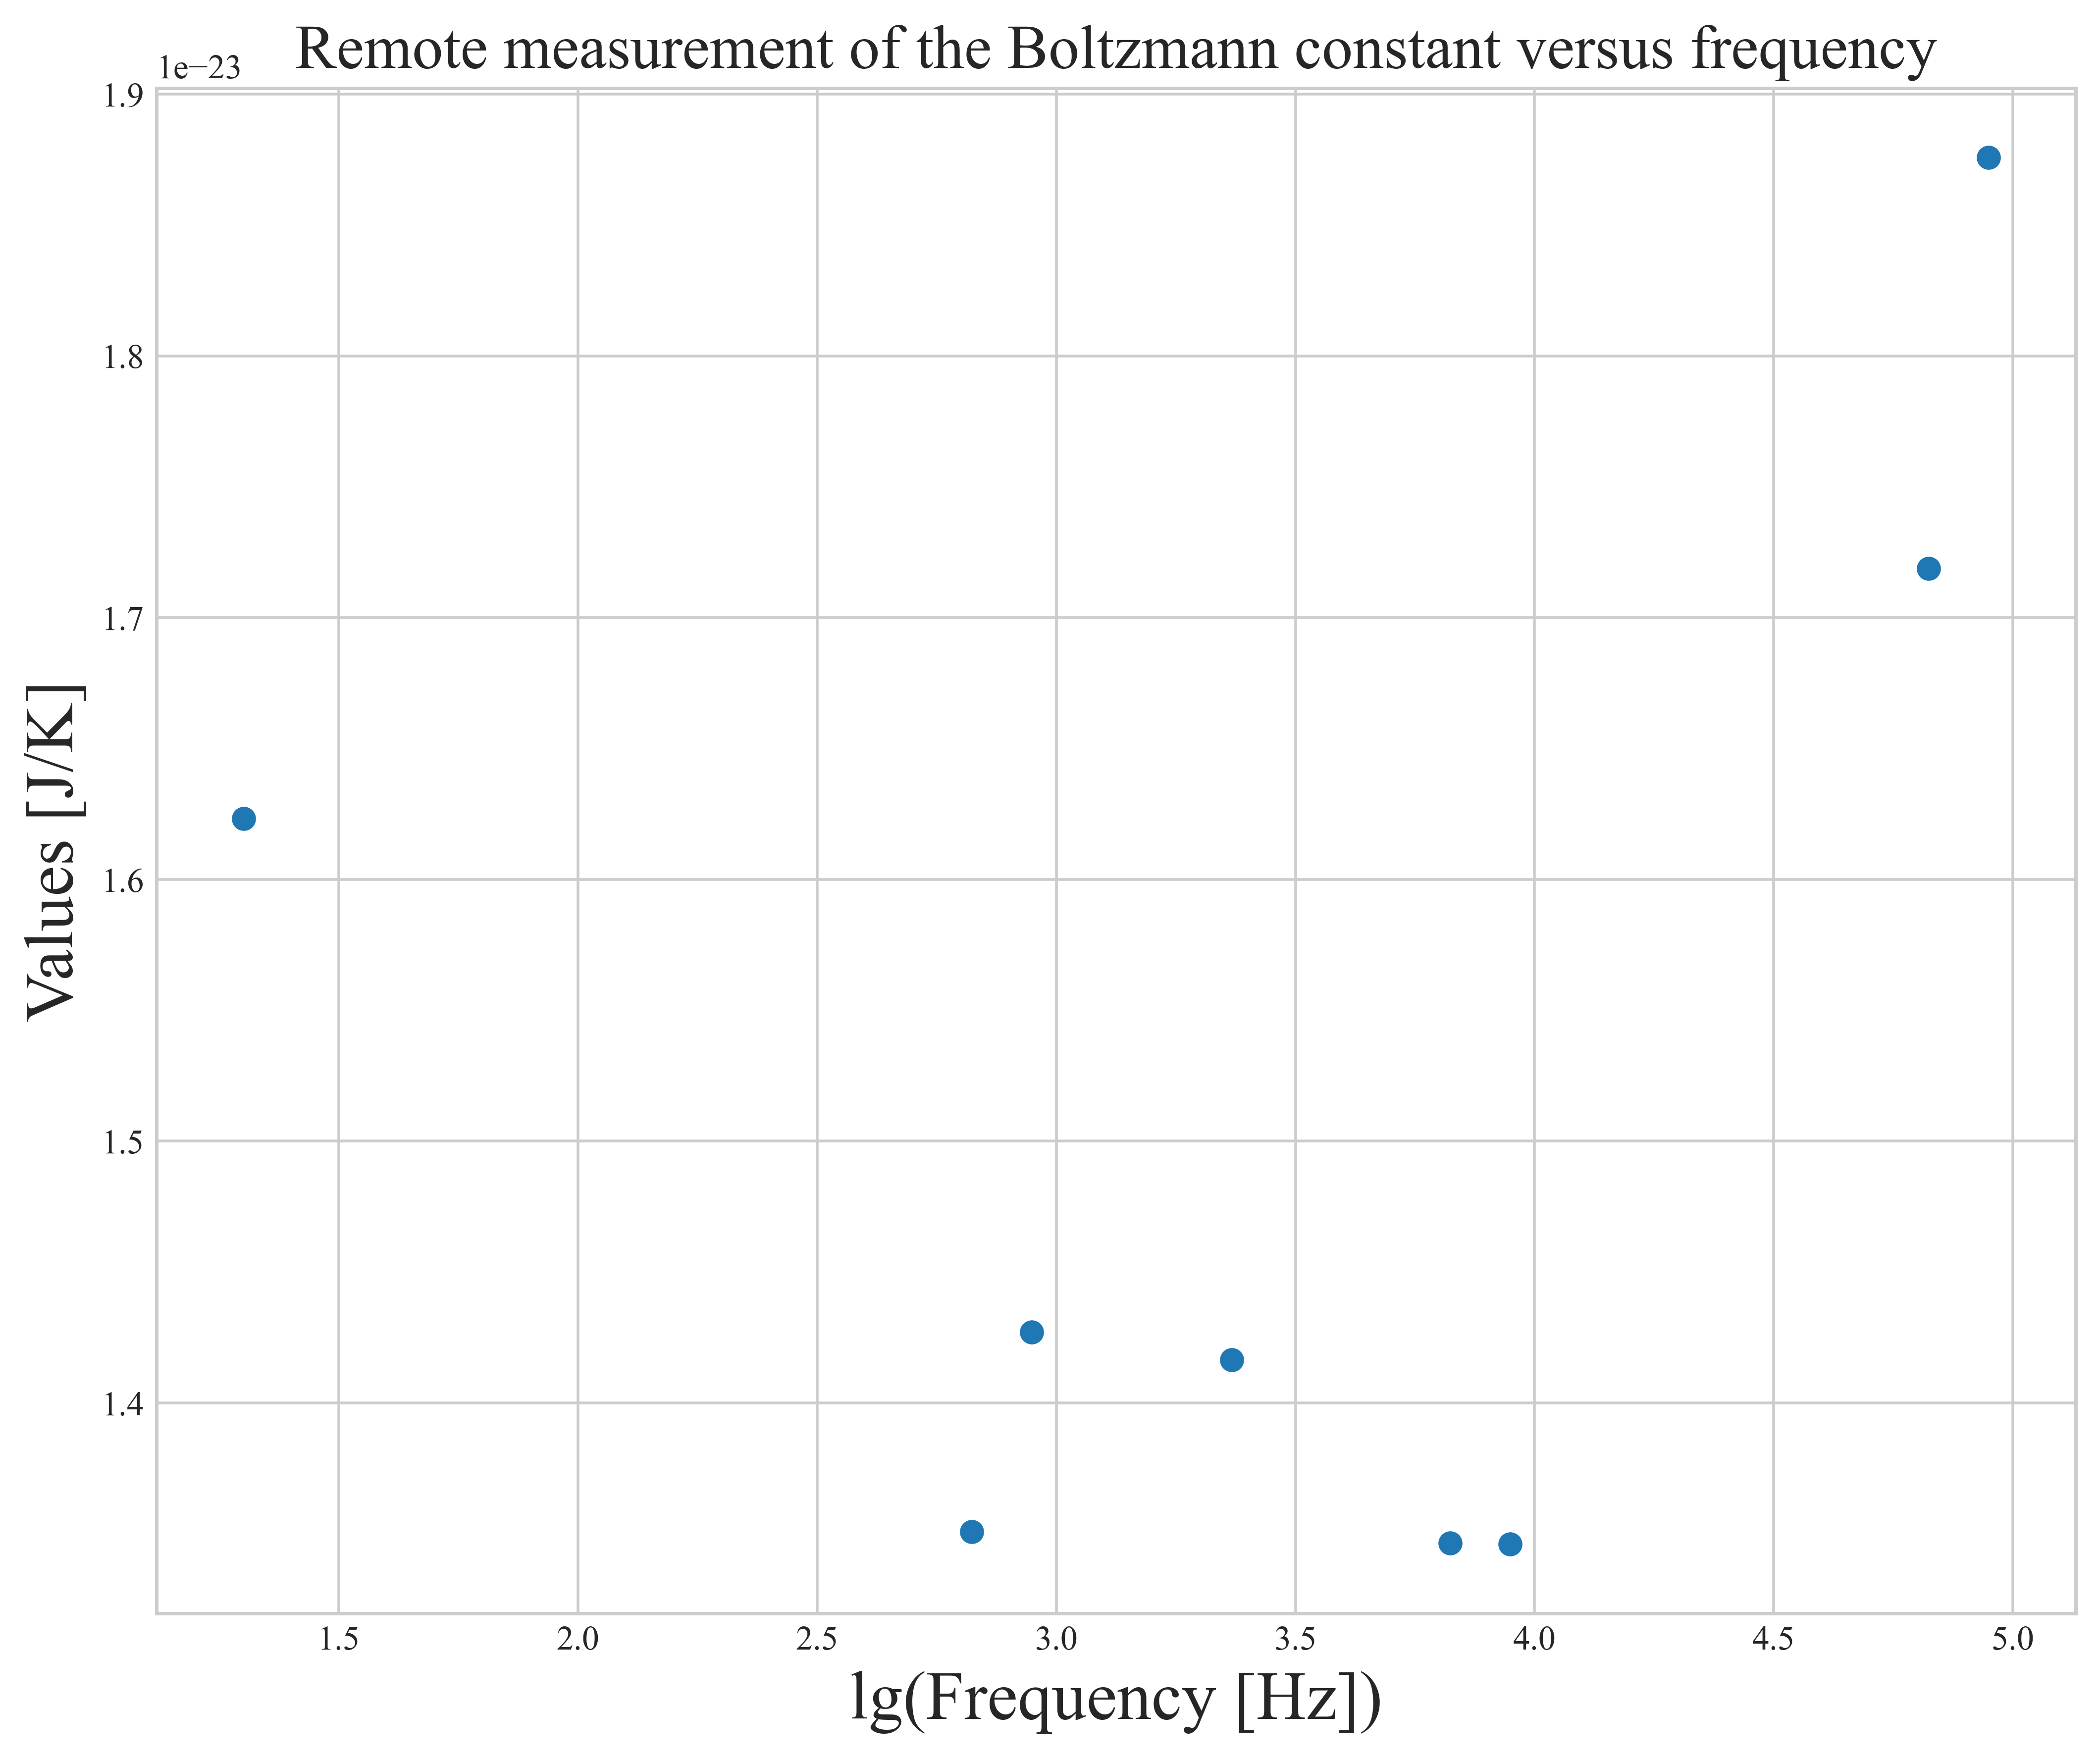
\includegraphics[width=0.7\linewidth]{images/APL1_1_A_kBf_remote}
		\caption{远程测量结果的频率分布}
		\label{fig:apl11akbfremote}
	\end{figure}
	
	考虑更详细的相关性检验，有：
	
	对数据“本地测量所得各玻尔兹曼常数测量值”进行相关性分析，结果如下所示：
	\begin{itemize}
		\item \textbf{Pearson Correlation Coefficient:}
		\begin{itemize}
			\item Coefficient: 0.9145, p-value: 0.0015
			\item 结论：在显著性水平 0.05 下，两列数据存在显著的线性相关性 (\( p \leq 0.05 \))
		\end{itemize}
		
		\item \textbf{Spearman Correlation Coefficient:}
		\begin{itemize}
			\item Coefficient: 0.7904, p-value: 0.0195
			\item 结论：在显著性水平 0.05 下，两列数据存在显著的非参数相关性 (\( p \leq 0.05 \))
		\end{itemize}
	\end{itemize}
	
	对数据“本地测量所得各玻尔兹曼常数测量值”进行相关性分析，结果如下所示：
	\begin{itemize}
		\item \textbf{Pearson Correlation Coefficient:}
		\begin{itemize}
			\item Coefficient: 0.8656, p-value: 0.0055
			\item 结论：在显著性水平 0.05 下，两列数据存在显著的线性相关性 (\( p \leq 0.05 \))
		\end{itemize}
		
		\item \textbf{Spearman Correlation Coefficient:}
		\begin{itemize}
			\item Coefficient: 0.2381, p-value: 0.5702
			\item 结论：在显著性水平 0.05 下，两列数据不存在显著的非参数相关性 (\( p > 0.05 \))
		\end{itemize}
	\end{itemize}
	
	\item 共用X和Y数据处理得到的$k_B$值求平均是否可以降低其随机误差？
	
	共用 \( X \) 和 \( Y \) 数据处理得到的玻尔兹曼常数 \( k_B \) 值取平均，确实可以有效降低随机误差。这是因为 \( X \) 和 \( Y \) 通道分别表示锁相放大器中相位上互差 90 度的两个正交信号分量，因此它们在测量时受到的随机噪声影响相对独立。通过分别计算 \( X \) 和 \( Y \) 得到的 \( k_B \) 值后取平均，可以减小噪声的标准差，降低随机误差。统计学上，独立测量值的平均能够有效降低方差，使最终结果的精度得到提升。此外，平均 \( X \) 和 \( Y \) 数据也可以部分抵消由于相位漂移或相位噪声带来的影响，从而提高测量结果的稳定性。最终，通过这种方式获得的 \( k_B \) 平均值可以更准确地反映实验结果，并减少随机误差对测量的干扰。
	
	\item 能否通过噪声谱密度计算不同频率下的$k_B$值及其算术平均值$\bar{k_B}$？
	
	虽然根据\cite{c}，我们得知是可以这样做的。但是基于前述对本实验的详细分析（\cref{fig:apl11akbflocal}和\cref{fig:apl11akbfremote}）我们可知由于未能得知是什么造成了测量值与频率存在关系而导致无法修正，\textbf{所以并不能这样做}。
	
	\item 本底噪声与仪器和测量时段有关， 输入带宽修正因子与电缆温度有关（参考\cite{c}）。
	
	我们实验所得的玻尔兹曼常数测量值如\cref{tab:kbvalues}所示，注意其中远程测量组我们在计算时并没有扣除本底噪声，可以发现它并没有为测量带来很大的干扰，因此在实验室人员活动少的时段本底噪声实际上是较小的（这也说明了我们本地测量得到的本底噪声很大一部分是当时较大的环境噪声）。
	
	此外，按\cite{c}，用阻抗分析仪测量 2m 长电缆分别在室温和一半在室温一半在液氮罐内的电容值，后者下降了约 30\%，对应式 $
	\frac{\delta v_{\text{BW}}}{v_{\text{BW}}} = 
	\left( 1 + \frac{n_{BX}^2}{n_{TX}^2} \right)
	\frac{ \left( \omega R_{\text{in}} C_{\text{in}} \right)^2 }{ 1 + \left( \omega R_{\text{in}} C_{\text{in}} \right)^2 }
	\left( \frac{\delta R_{\text{in}}}{R_{\text{in}}} + \frac{\delta C_{\text{in}}}{C_{\text{in}}} \right) $ 中的 $\delta C_{\text{in}} / C_{\text{in}} \approx -26\%$。由于样品电阻在液氮温度下需重新测量，且电缆电阻相对于样品电阻很小，因温度变化导致的 $\delta R_{\text{in}} / R_{\text{in}}$ 可以忽略。上式给出的输入带宽修正量在不同测量频率下和对不同样品电阻造成修正过度的程度不同，可解释液氮下 $k_B$ 测量值的离散系数大。
	
\end{enumerate}

%% 总结
%\subsubsection{Conclusion}
%\begin{itemize}
%	\item 
%\end{itemize}


%---------------------------------------------------------------------
% 实验后思考题
\subsection{Reflections after Experiment}
%思考题1
\begin{question}
	样品盒及传输电缆是否会对本底有贡献？ 用实验现象回答： 处于不同环境（如人的触碰、或插入液氮瓶后） 是否对测量产生影响？
\end{question}
\begin{enumerate}
	\item 实验中，样品盒和传输电缆确实会对本底噪声产生贡献。
	
	讲义提到，实验中的热噪声来源不仅限于电阻本身，还包括系统的各个部分。如果样品盒和电缆材料具有导电特性，则它们的热噪声会叠加在测量信号中。\textbf{传输电缆中的导线}在温度下会产生少量热噪声，这可能与锁相放大器检测到的电阻热噪声一起被测量到。样品盒与电缆连接处可能存在微小的\textbf{接触电阻}，而这种接触电阻在电流通过时会产生额外的噪声。此外，如果连接不稳定或接触不良，接触噪声的影响可能会更大。传输电缆可能在传输过程中\textbf{拾取环境中的电磁干扰}，如50Hz市电噪声或其他无线电信号。这些干扰信号会通过电缆进入测量系统，增加本底噪声水平。
	
	\textbf{本底噪声不必进行输入带宽修正}的原因在于其来源和特性。本底噪声主要是锁相放大器内部的固有噪声，包括仪器自身的电子噪声和散粒噪声等。由于这些噪声是仪器内部产生的，\textbf{它们的主要部分并不通过输入电路的阻容滤波}，因此不会受到输入带宽的影响。对于外部信号，如电阻的热噪声，由于其通过锁相放大器的输入电路进入测量系统，会受到输入阻抗和输入电容的影响，导致信号衰减。为了准确获得电阻的热噪声，必须通过带宽修正来还原信号的真实强度。
	
	\item 根据实验记录和讨论的内容​，不同环境条件（如触碰样品盒或将样品盒插入液氮瓶中）确实对测量结果产生了影响。这些环境因素可能会通过改变电缆和样品盒的电容值或引入额外的电磁干扰，从而影响本底噪声和信号的稳定性。例如，实验中提到在液氮瓶中的电缆电容比室温下降了约30\%（详见\textbf{误差分析}和\textbf{关于输入带宽修正的讨论}），而环境噪声在实验人员活动较多的时段也会增加。这些变化表明，实验中环境条件的不同会对噪声测量产生干扰，影响实验精度。
	
	\item 下面具体分析一个案例：我们实验所得的玻尔兹曼常数测量值如\cref{tab:kbvalues}所示，注意其中远程测量组我们在计算时并没有扣除本底噪声，可以发现它并没有为测量带来很大的干扰，因此在实验室人员活动少的时段本底噪声实际上是较小的（这也说明了我们本地测量得到的本底噪声很大一部分是当时较大的环境噪声）。
	
\end{enumerate}

% 思考题2
\begin{question}
	采样时间间隔$\Delta t$约多少个时间常数时，X任意相邻采样读数$X(t)$与$X(t+\Delta t)$可视独立无关的？如何验证？如想缩短测量时间并要求采样读数保持随机噪声特性，选择时间常数为多长合适？
\end{question}
\begin{itemize}
	\item 首先根据\cite{c}中结论，当$t_s=10\tau$时，无论是 X 或 Y 分量还是某单分量的噪声电压是无关的。
	
	\begin{figure}[h!]
		\centering
		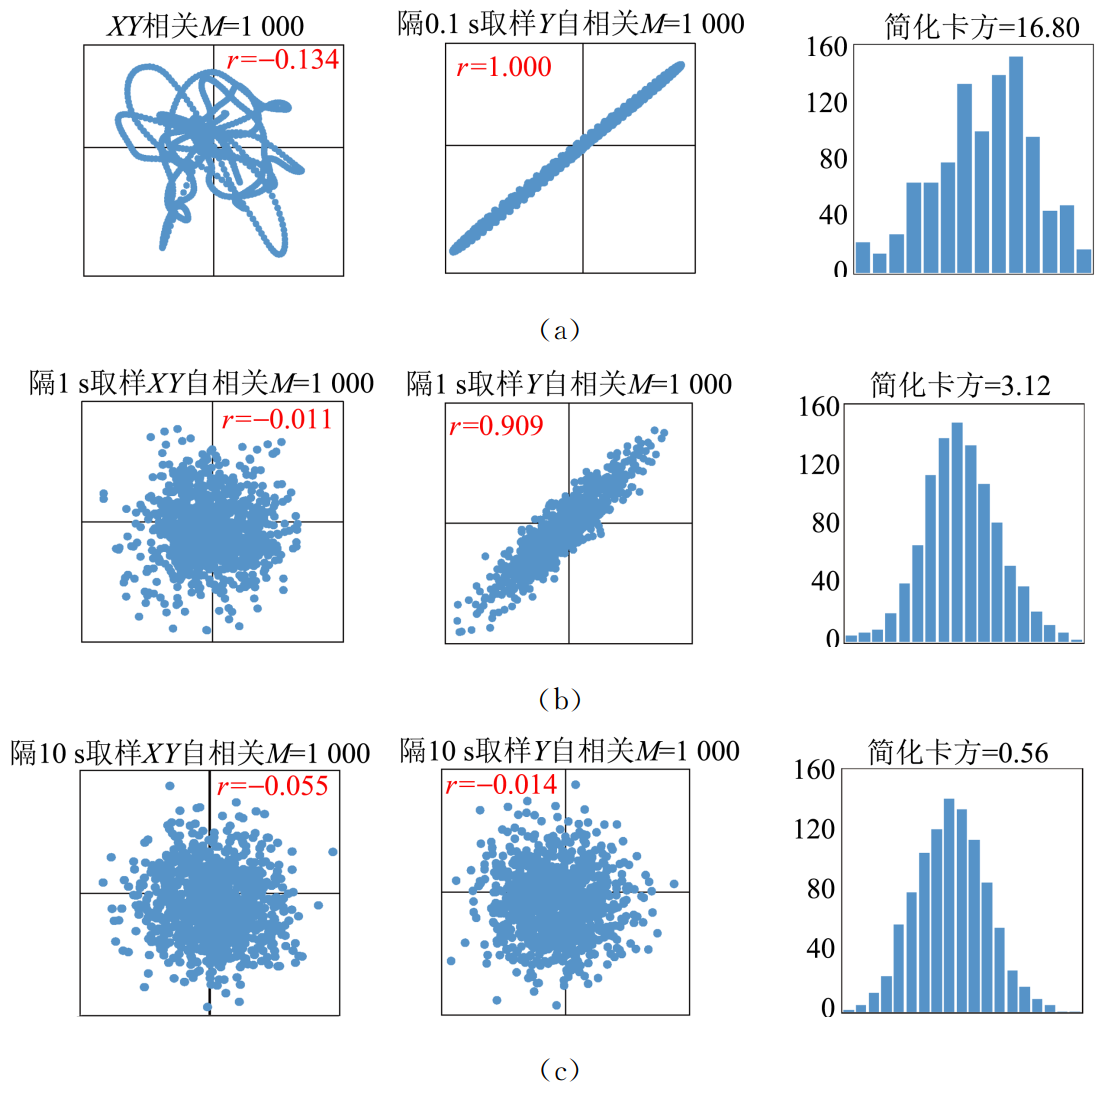
\includegraphics[width=0.6\linewidth]{images/APL1_1_A_tauts}
		\caption{采样间隔对数据相关性的影响（来自\cite{c}）}
		\label{fig:apl11atauts}
	\end{figure}
	
	\item 其次在我们的实验中，我们均使用的是$t_s=10\tau$的条件，该条件下按前述相关性分析的结果（\cref{fig:localdata1}，\cref{fig:localdata2}，\cref{fig:localdata3}，\cref{fig:remotedata4}和\cref{fig:remotedata9}），X任意相邻采样读数$X(t)$与$X(t+\Delta t)$都可视独立无关的。
	
	\item 从测量时间考虑：
	\begin{itemize}
		\item 现场测量实验时间从下午14:30到晚上18:00，有效测量时间小于两小时，测量8组数据点，每组数据点各至少1000个，因此考虑$\tau=10ms$，则$t_s=0.1s$，单组测量时间100s，理论总耗时800s约13min；结合本底测量时间、仪器接线时间、调试时间（试错时间）和数据分析时间，以及事实上我们每组的数据点远大于1000个，这个时间设置是较为合理的。
		
		\item 远程测量实验时间从晚上19:00到23:00，有效测量时间约3小时，选取$\tau=100ms$，则$t_s=1s$，单组测量时间1000s，同样测量共8组，每组至少1000个数据点，总耗时8000s约133min约2.2小时，这个时间设置也较为合理。
	\end{itemize}
\end{itemize}